\documentclass[11pt]{article}

% Change "review" to "final" to generate the final (sometimes called camera-ready) version.
% Change to "preprint" to generate a non-anonymous version with page numbers.

%  seems the only difference between preprint and final is the page numbers, so we can just use preprint.
\usepackage[preprint]{acl}
\usepackage{times}
\usepackage{latexsym}
\usepackage[T1]{fontenc}
\usepackage[utf8]{inputenc}
\usepackage{microtype}
\usepackage{inconsolata}
\usepackage{graphicx}
\usepackage{enumitem}
\usepackage{booktabs}
\usepackage{multirow}
\usepackage{placeins}
\usepackage{float}
\usepackage{balance}
% skip huge vertical space after title/author
\setlength\titlebox{8\baselineskip}




% Report requireements:
% ------------------------------- 
% max 8 pages

% General Note:
% - Whenever feasible, provide examples of the actual texts (tweets, blogs, sentences, reviews, etc.) that you reference. This will enhance the clarity and tangibility of your report.
% - If you generated a unique dataset, kindly submit it with your report (unless privacy concerns arise).
% - While you're welcome to submit any software you developed, note that we won't assess the quality of your programming.

% Assessment criteria:
% • Problem definition & motivation - clarity of the problem/question and its relevance.
% • Dataset - appropriateness, description, and transparency about limitations.
% • Methodology - correct application of NLP methods, clarity of explanation, and proper use of references/tools.
% • Experiments & results - sound setup, meaningful evaluation, and clear reporting of outcomes.
% • Discussion & conclusion - critical reflection on findings, limitations, and ethical aspects.
% • Presentation & writing - overall structure and readability.



% Citation commands for template: 
% ------------------------------- 
% \citet{key}      -> Author (year)           [cite in text]
% \citep{key}      -> (Author, year)          [cite in parentheses]
% \citealp{key}    -> Author, year            [alternative cite without parentheses]
% \citeyearpar{key}-> (year)                  [cite year only in parentheses]
% \citeposs{key}   -> Author's (year)         [possessive citation, ACL only]


\title{Hybrid Feature-Based Detection of AI-Generated Text}
\author{Finn Fonteijn \\
  \texttt{s2899078} \\
  \texttt{f.f.fonteijn@student.utwente.nl} \\
  \\\And
  Linn Gregussen \\
  \texttt{s3422372} \\
  \texttt{l.y.gregussen@student.utwente.nl} \\}


\begin{document}
\maketitle
\begin{abstract}
The proliferation of large language models necessitates reliable detection of AI-generated text in academic and journalistic contexts. This study investigates which linguistic features best distinguish human from AI-generated text (RQ1) and whether ensemble methods improve robustness (RQ2). We extract 40 linguistic and statistical features from 112,848 samples across four diverse datasets and train multiple classifiers. XGBoost achieves 97.62\% accuracy (0.997 AUROC) on within-dataset testing, but performance drops to 82.76\% on cross-dataset evaluation, revealing severe overfitting. In contrast, DeBERTa maintains 96.57\% accuracy across datasets (0.994 AUROC), demonstrating superior generalization. Perplexity emerges as the most discriminative feature across all models (importance: 0.334-0.430), with higher perplexity indicating human text. Our voting ensemble achieves 95.58\% within-dataset accuracy and 88.89\% cross-dataset accuracy, providing robust performance through classifier diversity. Results demonstrate that transformer-based approaches generalize substantially better than feature-based methods for practical deployment, though simple ensemble voting further enhances robustness across domains.
\end{abstract}

\section{Introduction}
\label{sec:introduction}
% State the specific problems you aimed to address or the questions you sought to answer. If your project was inspired by a particular paper (or papers), which motivated your interest in the problem, kindly reference them here.

The availability of large language models (LLMs) creates a demand for reliable detection of AI-generated text in domains such as academia and journalism. Recent surveys indicate that hybrid approaches to AI detection, combining statistical and neural methods, often outperform single-modality detectors in both robustness and generalization \citep{wu-etal-2025-survey, su2024robustdetectionllmgeneratedtext}. A recent study by \citet{erol2025trust} exemplifies these challenges in academic contexts, evaluating three commercial AI detectors on 250 human-written neurosurgery abstracts from pre-ChatGPT journals and 750 AI-generated versions (using ChatGPT 3.5, 4, and 4o). While the detectors achieved high AUC scores (0.96--1.00), they misclassified up to 30.4\% of human texts as AI-generated, raising ethical concerns about false accusations in peer review.

Motivated by such findings, this project takes a dual approach to AI text detection. First, we conduct a feature-based analysis to identify which linguistic and statistical patterns are most discriminative. Second, we implement an ensemble-based detector combining multiple classification approaches to explore whether such combinations can improve practical deployment robustness.

This project addresses two research questions:

\textbf{RQ1:} \textit{Which linguistic or statistical features are most effective in distinguishing human- vs. AI-generated text?}

\textbf{RQ2:} \textit{How does ensemble-based classification improve robustness compared to individual classifiers?}

\section{Related Work}
\label{sec:related-work}
% Although not an exhaustive literature review, discuss a few key papers that tackled similar problems. Highlight their data and methods, outcomes, and outline the points of distinction between your approach and theirs.
\citet{wu-etal-2025-survey} conducted a comprehensive review of the state-of-the-art in LLM-generated text detection in 2025. They classify LLM-generated text detectors into three categories: watermarking technology where the generator includes identifiable patterns in the text to regulate and detect its origin; statistics-based detectors which analyze inherent patterns of the generated text; and neural-based detectors which use machine learning models to classify the generated text. The detectors in the survey report performance using different metrics, but among the best performing are the two statistics-based detectors "Ghostbuster" with average F1 score of 99.0 and GECScore with an AUROC of 98.62\%. Among the neural-based detectors, DNA-GPT achieved "nearly 100\%" detection accuracy in distinguishing between human-written and GPT-generated texts on multiple datasets. The watermarking methods are noted for their robustness against adversarial attacks, e.g. reliable classification when up to 50\% of the tokens were modified, and low false-positive rates, making them a promising approach for reliable detection. 

However, robustness against adversarial attacks remains a significant challenge. \citet{weber-wulff_testing_2023} examine the reliability of AI text detection tools in academic settings and found that obfuscation techniques, e.g. manual editing and machine paraphrasing, significantly reduce the accuracy of detection tools, with approximately 50\% of the texts that had undergone some type of post-generation editing being misclassified as human-written. Similar results, with detectors being less accurate when subjected to adversarial attacks, are reported by \citet{wu-etal-2025-survey} and \citet{pudasaini_survey_2025}. 

Multiple surveys indicate that hybrid approaches, combining statistical and neural methods, often outperform single-modality detectors in robustness and generalization \citep{wu-etal-2025-survey, su2024robustdetectionllmgeneratedtext}.

\section{Data}
\label{sec:data}
% Describe the dataset employed in your project. Explain dataset properties, its composition (documents, sentences, words), and labelling information (by whom, how).Indicate the source if it's an existing dataset, or if you created your own, describe the process.

To ensure our model generalizes across diverse English language sources, domains, and LLMs, and to mitigate overfitting to any single dataset's biases, we utilize multiple datasets for training and evaluation. This approach allows for robust testing of features and hybrids in varied contexts. The datasets include AH\&AITD (Arslan's Human and AI Text Database) with texts across domains including articles, abstracts, stories, news, and reviews \citep{akram2023ahaitd}; the LLM - Detect AI Generated Text Dataset (Kaggle sunilthite) containing essays \citep{thite2023llm}; the DAIGT V2 Train Dataset (Kaggle) with essays \citep{deotte2023daigtv2}; and the Human ChatGPT Comparison Corpus (HC3) comprising Q\&A from domains such as finance, medicine, law, and open-domain questions \citep{guo-etal-2023-hc3}.

\subsection{Dataset Balancing}
\label{sec:dataset-balancing}
The datasets showed varying degrees of class imbalance between the target classes human-written (0) and AI-generated (1), ranging from 31.5\% AI-generated in the HC3 dataset to 50.0\% AI-generated in the AH\&AITD dataset. Dataset class distributions are detailed in Appendix \ref{sec:dataset-details}.

The dataset was balanced using a per-source strategy, where each source contributes an equal number of human-written and AI-generated samples according to its configured proportion of the total dataset size, and limited by the smallest class per source. This ensures balanced representation across both the source datasets and the target classes. Building on this balanced dataset foundation, we now describe our methodological approach for AI text detection, which combines feature-based analysis with ensemble-based classification.

\section{Method}
\label{sec:method}
% Clearly describe the method you employed to address your problem. Mention any libraries utilised, and ensure your explanation is accessible to individuals with fundamental NLP knowledge. Reference relevant literature where applicable. Additionally, mention preprocessing steps and dataset division into training and testing sets (if applicable).

The project methodology consists of two efforts to address different aspects of AI text detection: a feature-based analysis and an ensemble-based detector.

\subsection{Approach 1: Feature-Based Analysis}
\label{sec:feature-based-analysis}
The feature-based analysis focuses on understanding which linguistic and statistical features are most informative in classifying human- vs. AI-generated text. For each text in the dataset, a set of features are extracted (section \ref{sec:feature-extraction}). These features are then used to train three lightweight classifiers: logistic regression and random forest using scikit-learn \citep{scikit-learn}, and XGBoost \citep{xgboost}.

The dataset was balanced as described in section \ref{sec:dataset-balancing}. Feature importance rankings were retrieved and compared across these three models, giving insights on which linguistic patterns are consistently important for distinguishing human- vs. AI-generated text.

\subsubsection{Feature Extraction}
\label{sec:feature-extraction}
For each entry in the dataset, the following features were extracted using the spaCy library \citep{spacy} with the \texttt{en\_core\_web\_sm} model for all linguistic processing tasks, including tokenization, lemmatization, part-of-speech tagging, and dependency parsing.

\paragraph{Lexical Features}
Four lexical features were chosen and extracted. Average word length and word length variance to measure vocabulary complexity. Root Type-Token Ratio (RTTR), and hapax legomena ratio to measure lexical diversity.

The Root Type-Token Ratio (RTTR) is a token-type ratio that accounts for document size by normalizing by the square root of the document length \citep{REVIRIEGO2024100602}, defined as RTTR = Types / $\sqrt{\mathrm{Tokens}}$. It was calculated by lemmatizing the text, counting the unique types and dividing by the square root of text length. A hapax legomenon refers to a word (or expression) occurring only once in a context, and here measures the proportion of words that appear exactly once in a sample.

\paragraph{Syntactic Features}
Sentence-level statistics were chosen to measure sentence complexity, and include average sentence length and variance. Parse tree depth features (average, maximum and variance) were extracted to measure syntactic complexity. Parse depth is computed as the maximum number of ancestors for any token in a sentence.

\paragraph{Punctuation Features}
The ratio of punctuation marks to word count was calculated for comma, period, exclamation mark, and question mark. Additionally, the overall punctuation ratio was included.

\paragraph{Part-of-Speech Features}
POS tags were extracted using spaCy's coarse-grained POS tags (\texttt{token.pos\_}) rather than fine-grained tags (\texttt{token.tag\_}) to capture overall patterns in word class usage, fine grained tags were excluded as they may be too specific for the objective, and yield sparse data. The ratio of each POS category (noun, verb, adjective, adverb, etc.) to total tokens was calculated as well as a noun-to-verb ratio as a derived feature.

\paragraph{Perplexity}
Perplexity is defined as $\mathrm{PPL} = \exp\left(-\frac{1}{N}\sum_{i=1}^N \log p(w_i)\right)$, where $N$ is the number of tokens and $p(w_i)$ is the model's predicted probability for token $i$ \citep{jm3}. It measures how ``surprised'' the model is by the text: lower perplexity indicates more predictable text for the model. Perplexity was calculated using EleutherAI's Pythia 1.4B model \citep{biderman2023pythia}, an open-source model trained on the Pile dataset \citep{pile}. Pythia was specifically chosen for its reproducibility and transparency in training, providing deduplicated data variants that ensure clean perplexity signals without contamination artifacts from memorized training data \citep{biderman2023pythia}. This makes it ideal for AI text detection where we need to distinguish true predictive patterns from artificial recognition of memorized content.

\paragraph{Burstiness Features}
In statistics, burstiness is a measure of the variability in data points over time. Burstiness captures the "clumpiness" in text structure, where AI text might show more uniform patterns while human writing exhibits greater variation. The core burstiness metric uses the Goh-Barabasi coefficient \citep{Goh_2008}: \(B = \frac{\sigma - \mu}{\sigma + \mu}\), where \(\sigma\) is the standard deviation and \(\mu\) is the mean, this measure is designed for analyzing variation in sequential data distributions, which is what we wish to analyze. The formula yields a burstiness score between -1 (uniform) and 1 (highly variable). For each text input, ten burstiness features were originally extracted, measuring variation at the sentence, word, and clause levels, including sentence length burstiness, positional variation (comparing first and second halves) and clause length burstiness. After correlation analysis, six burstiness features were retained.


\subsubsection{Feature Selection}
\label{sec:feature-selection}
To reduce collinearity, a correlation analysis was performed on all the described extracted features, and from pairs with high pairwise correlation ($r > 0.8$), one feature was dropped. The feature to be dropped was selected based on whether it was correlated with more other features, and which feature would be more informative in the project context. After this selection process, 40 linguistic and statistical features were left for model training. The list of selected and dropped features is shown in Table \ref{tab:feature-selection}, for the extended list with all POS-tags, see Appendix \ref{sec:full-list-of-features}.

\begin{table}[t]
  \centering
  \caption{List of selected/considered linguistic features (40 features total). Dropped features (marked with †) were selected for redundancy while prioritizing informativeness.}
  \footnotesize
  \begin{tabular*}{\columnwidth}{@{\extracolsep{\fill}}ll}
  \toprule
  \textbf{Category} & \textbf{Feature Name} \\
  \midrule
  \multirow{4}{*}{Lexical}
   & average\_word\_length \\
   & word\_length\_variance \\
   & rttr\_root\_type\_token\_ratio \\
   & hapax\_legomena\_ratio \\
  \midrule
  \multirow{5}{*}{Syntactic}
   & average\_sentence\_length \\
   & sentence\_length\_variance \\
   & average\_parse\_depth \\
   & maximum\_parse\_depth \\
   & parse\_depth\_variance \\
  \midrule
  \multirow{5}{*}{Punctuation}
   & comma\_ratio \\
   & period\_ratio \\
   & exclamation\_mark\_ratio \\
   & question\_mark\_ratio \\
   & punctuation\_per\_word \\
  \midrule
  \multirow{2}{*}{Part-of-Speech (POS)}
   & pos\_ratio\_<tag> \\
   & noun\_to\_verb\_ratio \\
  \midrule
  \multirow{7}{*}{Burstiness}
   & sentence\_length\_burstiness \\
   & sentence\_length\_iqr \\
   & position\_burstiness\_diff \\
   & long\_sentence\_ratio \\
   & word\_length\_burstiness \\
   & clause\_length\_burstiness \\
   & \textit{sentence\_length\_cv}\textsuperscript{†} \\
   & \textit{sentence\_length\_range\_ratio}\textsuperscript{†} \\
   & \textit{adjacent\_sentence\_variation}\textsuperscript{†} \\
   & \textit{short\_sentence\_ratio}\textsuperscript{†} \\
  \midrule
  Other & perplexity \\
  \bottomrule
  \multicolumn{2}{l}{\footnotesize\textsuperscript{†} Removed; high correlation ($r>0.8$) with other feature(s)}
  \end{tabular*}
  \label{tab:feature-selection}
  \end{table}


\subsection{Approach 2: Ensemble-Based Detector}
\label{sec:ensemble-based-detector}
The ensemble-based detector combines five classifiers to build a practical, robust AI text detector. The classifier outputs are combined using two methods: majority voting and stacking.

\subsubsection{Base Classifiers}
\label{sec:base-classifiers}

The ensemble-based detector is made up of multiple text-based classifiers and the XGBoost classifier from Approach 1 (Section \ref{sec:feature-based-analysis}) leveraging different perspectives on the classification task. 

\paragraph{BERT Classifier}
BERT captures contextual word representations through its bidirectional transformer architecture, letting it capture semantic patterns in text.
For this project the BERT classifier available at Hugging Face as \texttt{google-bert/bert-base-uncased} is used \citep{devlin2019bertpretrainingdeepbidirectional}.

\paragraph{DeBERTa Classifier}
A DeBERTa-based classifier using the \texttt{microsoft/deberta-v3-base} model. DeBERTa uses disentangled attention mechanisms and enhanced mask decoder, this way a word's content can be separated from its position and processed independently, this gives it a clearer sense of what's being said and where in the sentence it's happening, potentially capturing more nuanced linguistic patterns for the AI classification task \citep{he2023debertav3improvingdebertausing}.


\paragraph{Naive Bayes Classifiers}
Two Naive Bayes classifiers were included in the ensemble, one using the full vocabulary and one with stopwords removed.

\paragraph{XGBoost Classifier}
The XGBoost classifier described in section \ref{sec:feature-based-analysis} was also added to the ensemble, giving the ensemble access to the explicit linguistic features extracted from the text.

\subsubsection{Ensemble Methods}
\label{sec:ensemble-methods}
Two ensemble methods were implemented: majority voting and stacking.

\paragraph{Majority Voting}
In the voting approach, each of the five base classifiers independently predicts the class label for a given text. The final prediction of the ensemble is then determined by a majority vote across the classifiers. This simple aggregation reduces individual model errors, increasing robustness against the misclassification of a single model.

\paragraph{Stacking}
In the stacking approach, the predictions of all base classifiers on the training set are used as features to train a final estimator model. Three models were tested for this final estimator: Logistic Regression, Random Forest, and XGBoost, all implemented using the scikit-learn library \citep{scikit-learn}. Like majority voting, individual errors are reduced, but the use of a final estimator allows the ensemble to learn optimal weights for the different classifiers, potentially improving the overall performance of the ensemble. 


\subsection{Evaluation}
\label{sec:evaluation}

\subsubsection{Evaluation Strategy}
To distinguish between optimistic within-distribution performance and real-world generalization, we employ two complementary evaluation approaches.

\textbf{Within-dataset evaluation} uses an 80/20 stratified train-test split on the combined balanced dataset, establishing performance upper bounds when training and deployment distributions align.

\textbf{Cross-dataset evaluation} employs leave-one-dataset-out cross-validation: training on three source datasets and testing on the fourth held-out dataset (10,000 samples per test). This stringent approach reveals whether models learn generalizable linguistic patterns or merely overfit to dataset-specific artifacts. The substantial distribution shift simulates real-world deployment where text sources are heterogeneous, providing a realistic assessment of practical reliability.

\subsubsection{Classification Metrics} All classifiers are evaluated on a held-out test set using multiple performance metrics: accuracy, precision, recall, F1-score (macro, weighted, and per-class), and AUROC (Area Under the ROC Curve). AUROC provides a threshold-independent measure of classifier performance across all classification thresholds (0-1, with higher values indicating better discrimination between classes), with random baseline performance at 0.5. For the ensemble, both individual model performance and complete ensemble performance are reported, to allow comparison between the internal ensemble methods and the overall ensemble performance.

\subsubsection{Feature Importance Analysis} For the feature-based analysis, we extract and compare feature importances from each model: absolute coefficient values from logistic regression (normalized to sum to 1), Gini importance from random forest, and gain-based importance from XGBoost. By ranking features across models, we identify which linguistic patterns are consistently discriminative regardless of the classification algorithm.

\paragraph{SHAP Summary Plots}
SHAP (SHapley Additive exPlanations) values are calculated and visualized for the XGBoost classifier to provide interpretable explanations of feature contributions using the shap library \citep{shap_library}. The SHAP summary plot visualizes the distribution and magnitude of each feature's impact across all test predictions by the XGBoost model, showing which features are most influential for the model's decisions, and in which direction.

\section{Experimental Setup}
\label{sec:experiment-setup}
The complete implementation of this project is available in the github repository nlp-ai-detector \citep{githubrepository}.

\subsection{Dataset Configuration}
The combined dataset consisted of 112,848 samples from the datasets described in Section \ref{sec:data} and was balanced per source and per class as described in Section \ref{sec:dataset-balancing}. Dataset composition is detailed in Appendix \ref{sec:dataset-details}. The data was split into training (80\%) and test (20\%) sets using stratified sampling with a fixed seed to ensure reproducibility and maintain class balance across splits, giving 90,278 training samples and 22,570 test samples.

\subsection{LLM Setup}
The LLM-models were downloaded from Hugging Face, and run using the transformers library \citep{wolf-etal-2020-transformers}. 
The models were configured with the following hyperparameters:

\paragraph{Feature-Based Classifiers}
Logistic Regression used default scikit-learn parameters with random state 42. Random Forest was configured with max depth 10 and random state 42. XGBoost used 100 estimators, max depth 6, learning rate 0.1, random state 42, and eval metric 'logloss'.

\paragraph{Transformer-Based Classifiers}
BERT (\texttt{google-bert/bert-base-uncased}) and DeBERTa (\texttt{microsoft/deberta-v3-base}) classifiers were configured identically: maximum sequence length 128 tokens, 3 training epochs, learning rate 0.005, batch size 64. For both models, pre-trained embeddings were frozen and only a linear classification head was trained.

\paragraph{Naive Bayes Classifiers}
Both Naive Bayes classifiers used alpha smoothing parameter 1.0 and bag-of-words features with CountVectorizer. The first used the full vocabulary, while the second had 'english' stopwords removed.

\paragraph{Ensemble Configuration}
The majority voting ensemble used unweighted voting across the five base classifiers. For stacking, all meta-classifiers Logistic Regression, Random Forest, and XGBoost, used library default parameters.

\paragraph{Perplexity Calculation}
Perplexity features were computed using the \texttt{EleutherAI/pythia-1.4b} model with a maximum sequence length of 1,536 tokens and a stride of 1,536 to avoid overlapping windows.

% \FloatBarrier
\section{Results}
\label{sec:results}

\subsection{Feature-Based Classifiers}

\paragraph{Classification Performance}
Table \ref{tab:feature-based-results} presents the performance of the three feature-based classifiers on the test set (22,570 samples, 11,285 per class). XGBoost achieved the highest performance with 97.62\% accuracy and 0.997 AUROC, followed by Random Forest (96.06\% accuracy, 0.993 AUROC) and Logistic Regression (92.82\% accuracy, 0.972 AUROC). 
\begin{table}[t]
\centering
\footnotesize
\resizebox{\columnwidth}{!}{%
\begin{tabular}{@{}lccc@{}}
\toprule
\textbf{Metric} & \textbf{Logistic Regr.} & \textbf{Random Forest} & \textbf{XGBoost} \\
\midrule
Accuracy & 0.928 & 0.961 & \textbf{0.976} \\
AUROC & 0.972 & 0.993 & \textbf{0.997} \\
\midrule
\multicolumn{4}{@{}l}{\textit{Human-Written}} \\
Precision & 0.931 & 0.949 & \textbf{0.969} \\
Recall & 0.925 & 0.973 & \textbf{0.980} \\
F1-Score & 0.928 & 0.961 & \textbf{0.975} \\
\midrule
\multicolumn{4}{@{}l}{\textit{AI-Generated}} \\
Precision & 0.926 & 0.973 & \textbf{0.980} \\
Recall & 0.931 & 0.948 & \textbf{0.969} \\
F1-Score & 0.928 & 0.960 & \textbf{0.974} \\
\midrule
F1 (Macro) & 0.928 & 0.961 & \textbf{0.975} \\
F1 (Weighted) & 0.928 & 0.961 & \textbf{0.975} \\
\bottomrule
\end{tabular}
}
\caption{Performance metrics for feature-based classifiers. Best values in bold.}
\label{tab:feature-based-results}
\end{table}

\paragraph{Feature Importance Analysis}
Figures \ref{fig:lr-features}, \ref{fig:rf-features}, and \ref{fig:xgb-features} show the top 10 features for each classifier. Perplexity dominates across all models (importance 0.334-0.430), followed by lexical features (average word length, hapax legomena ratio). The models show differences in which type of features are more discriminative: Logistic Regression and Random Forest emphasize syntactic complexity (four syntactic features each), while XGBoost relies more heavily on POS ratios (four POS features vs. one for LR and none for RF).

\begin{figure}[t]
\centering
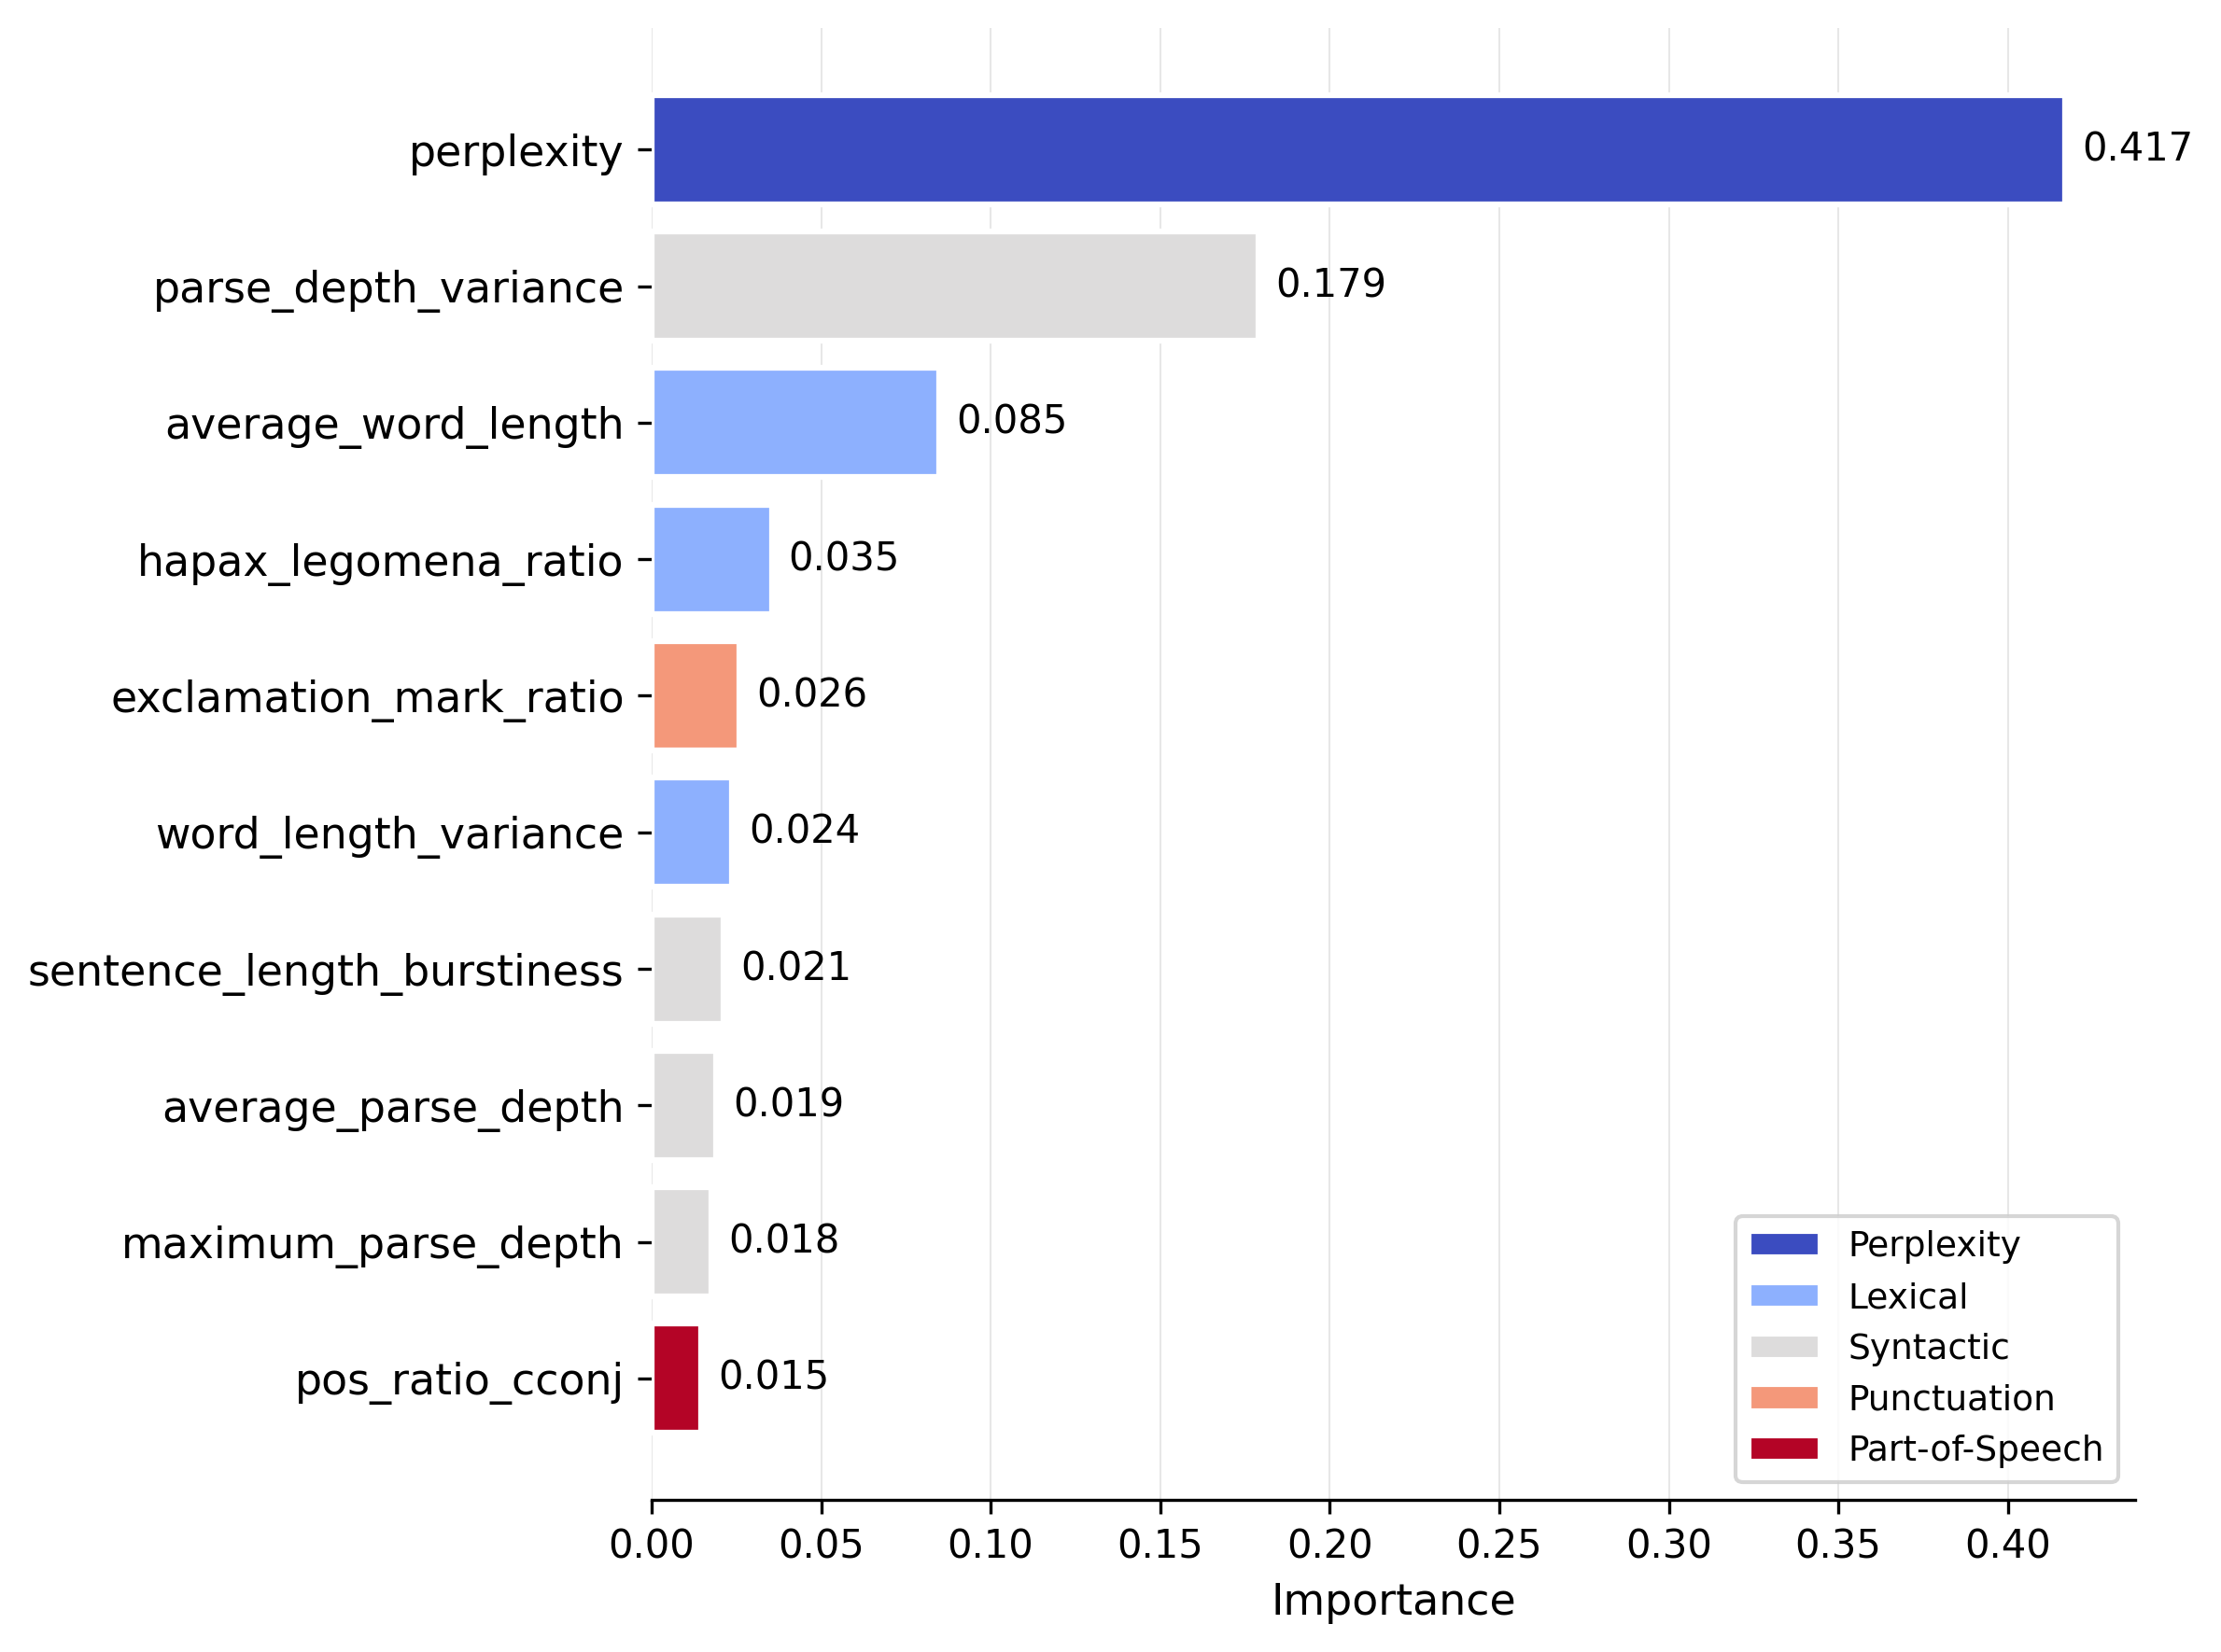
\includegraphics[width=0.8\columnwidth]{../plots/logistic_regression_features.png}
\caption{Top 10 feature importances for Logistic Regression classifier}
\label{fig:lr-features}
\end{figure}

\begin{figure}[t]
\centering
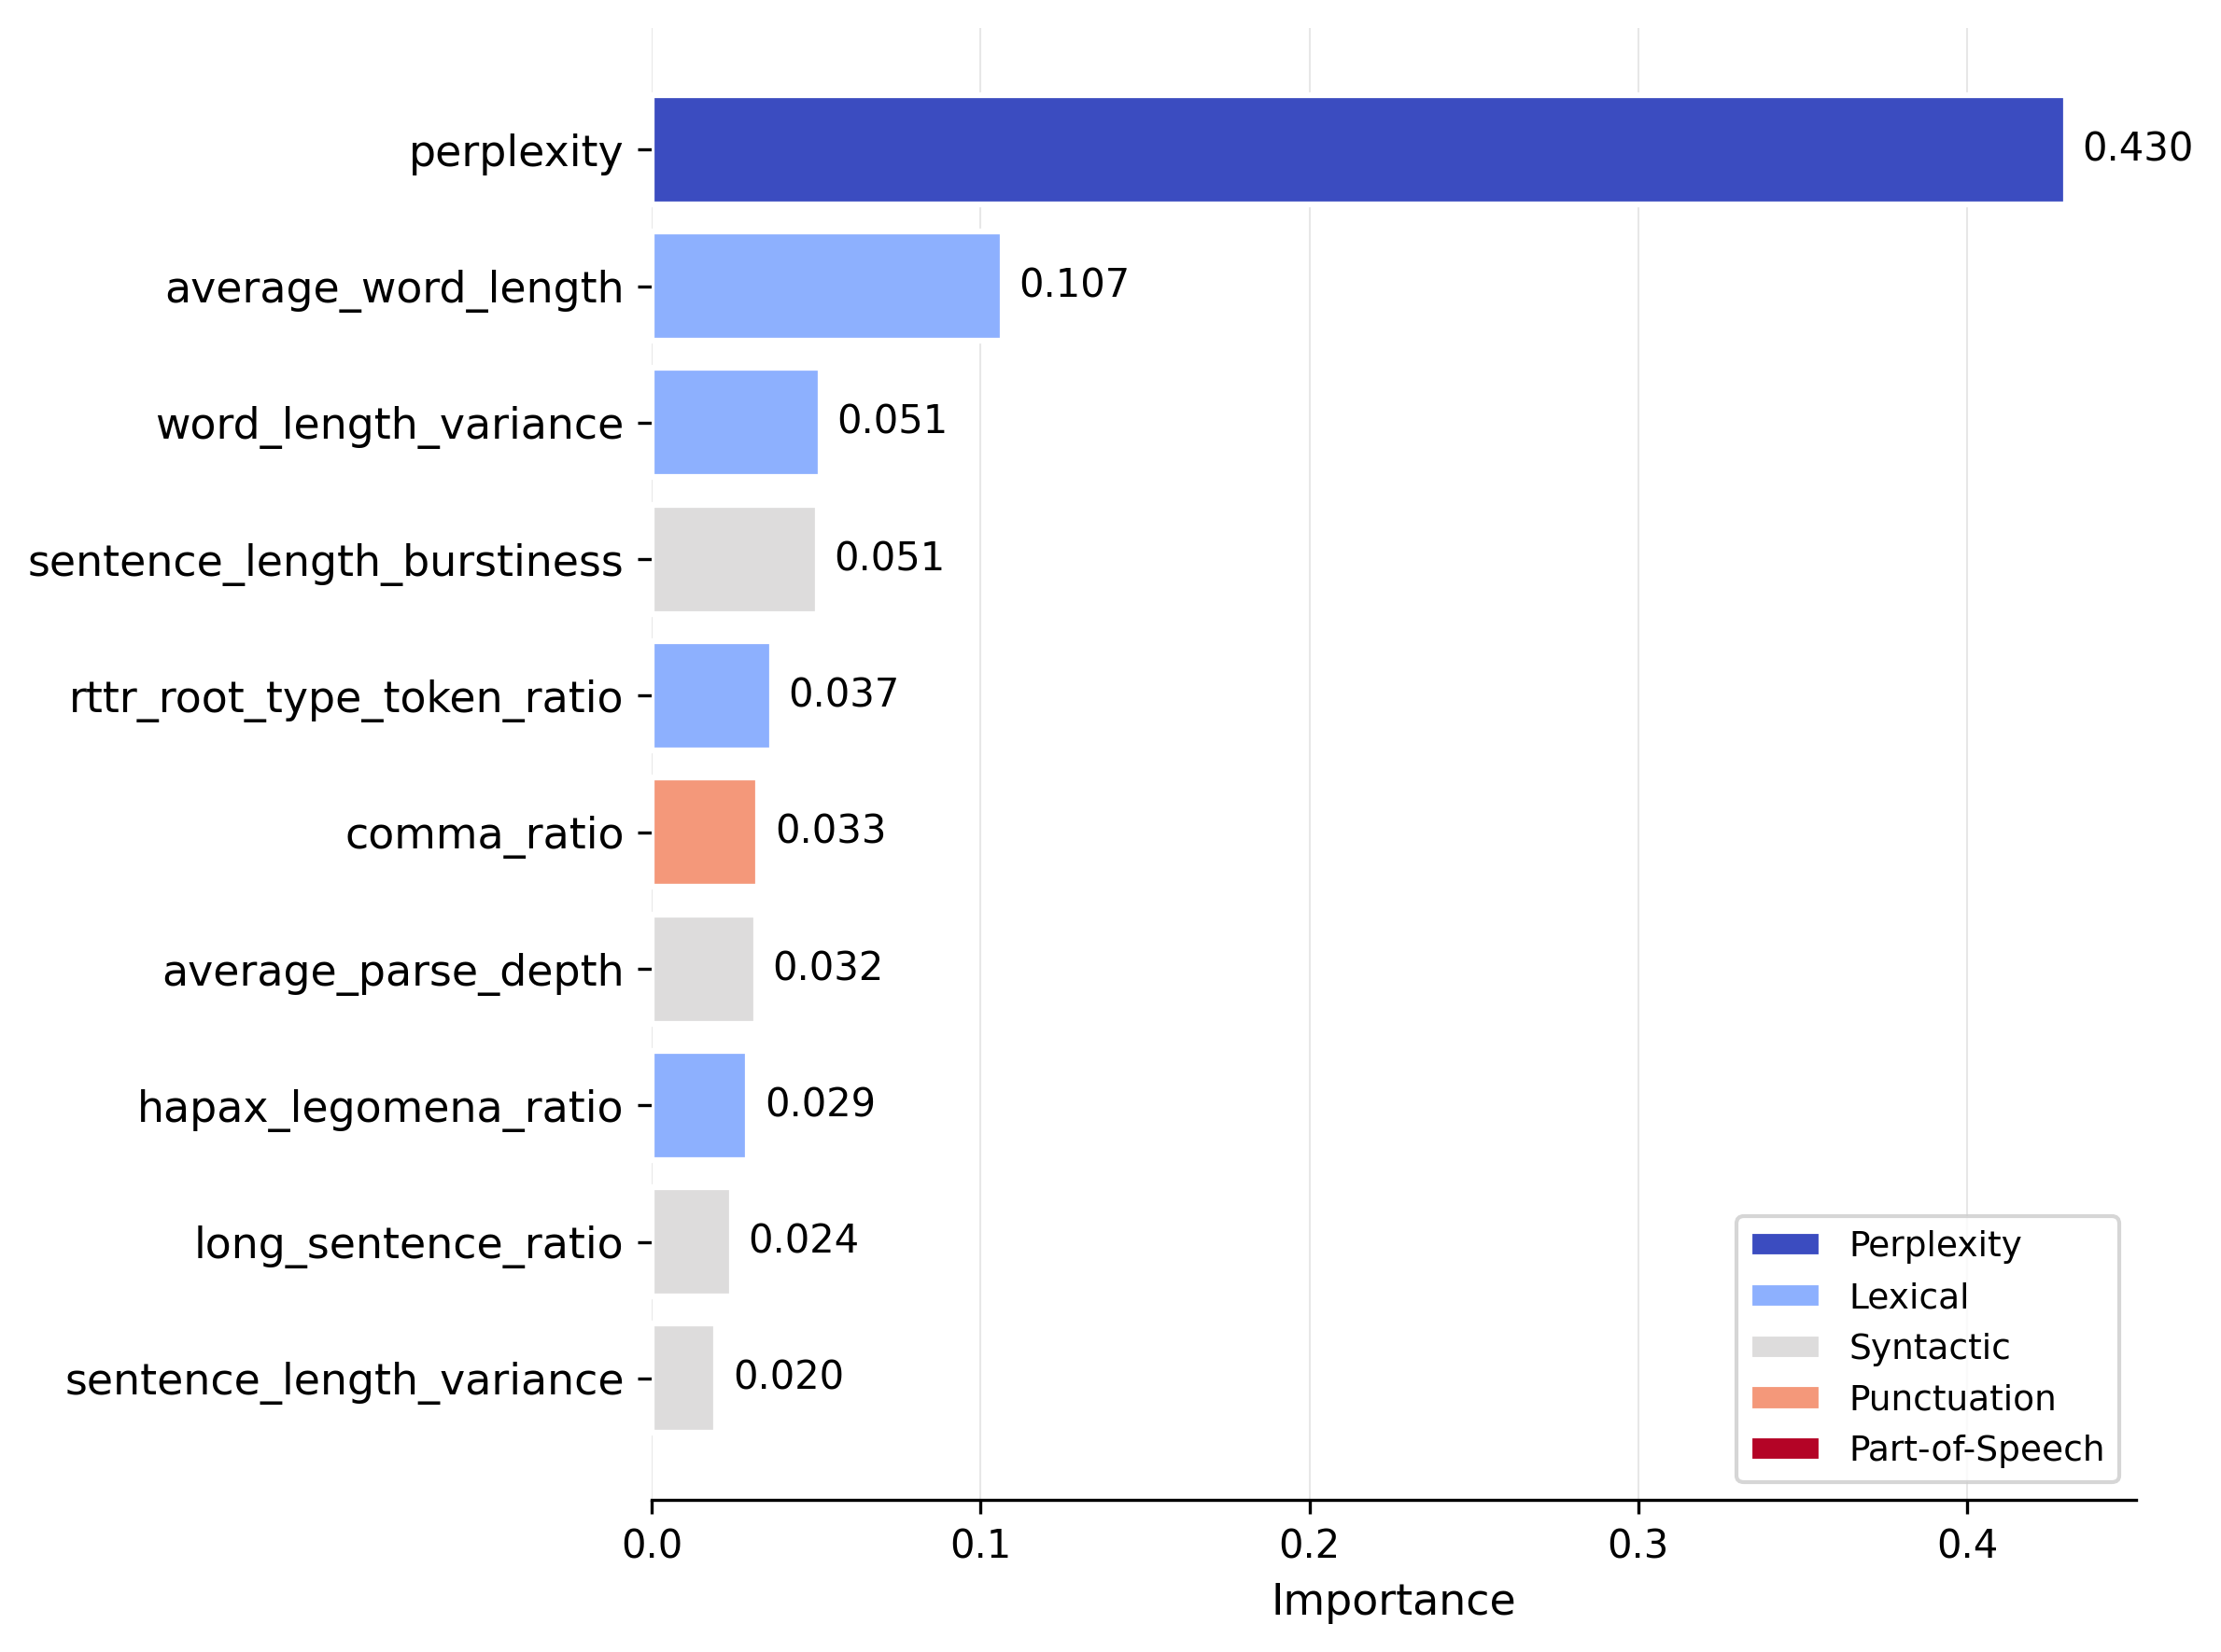
\includegraphics[width=0.8\columnwidth]{../plots/random_forest_features.png}
\caption{Top 10 feature importances for Random Forest classifier}
\label{fig:rf-features}
\end{figure}

\begin{figure}[t]
\centering
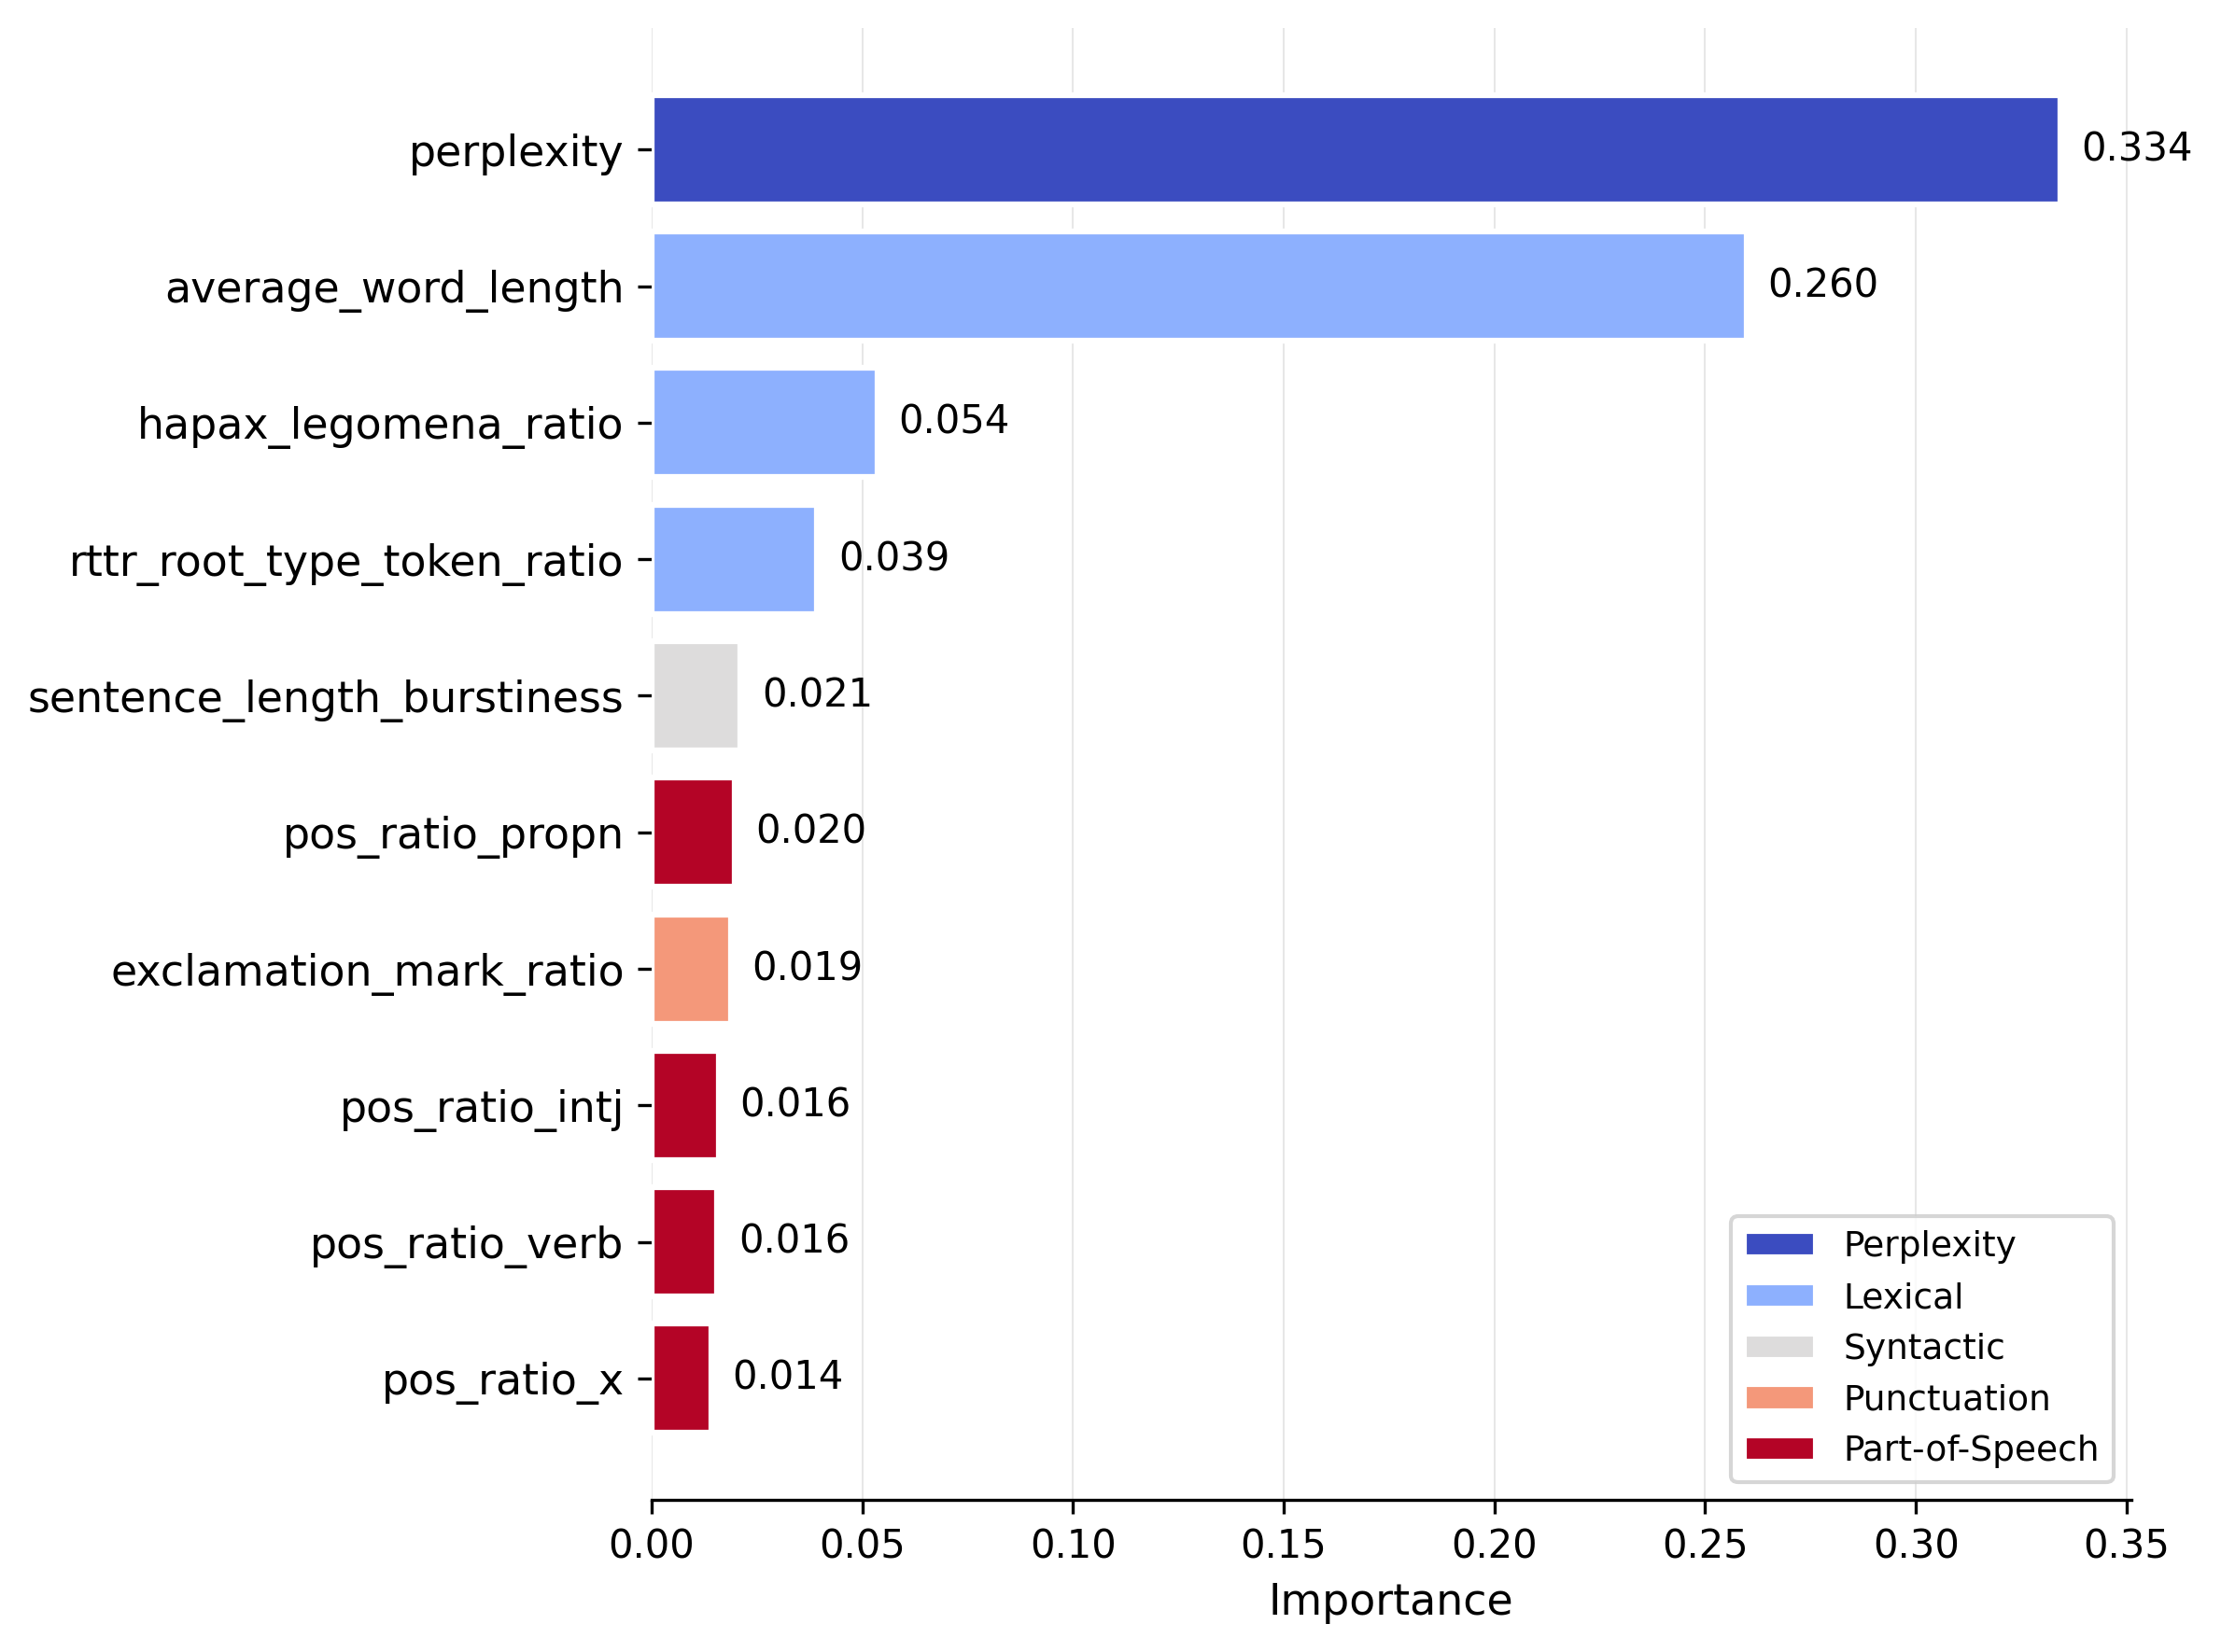
\includegraphics[width=0.8\columnwidth]{../plots/xgboost_features.png}
\caption{Top 10 feature importances for XGBoost classifier}
\label{fig:xgb-features}
\end{figure}


\paragraph{SHAP Summary Plot}
Figure \ref{fig:shap-summary} shows the SHAP analysis for the XGBoost classifier. Perplexity is the most discriminative feature, followed by lexical features (hapax legomena ratio, average word length, RTTR). High perplexity values (red) are strongly associated with human-written text, while low perplexity (blue) is strongly associated with AI-generated text. For the lexical features, lower values are associated with human-written text, that is less unique words, shorter words and a smaller range of words is associated with human-written text.

\begin{figure}[t]
\centering
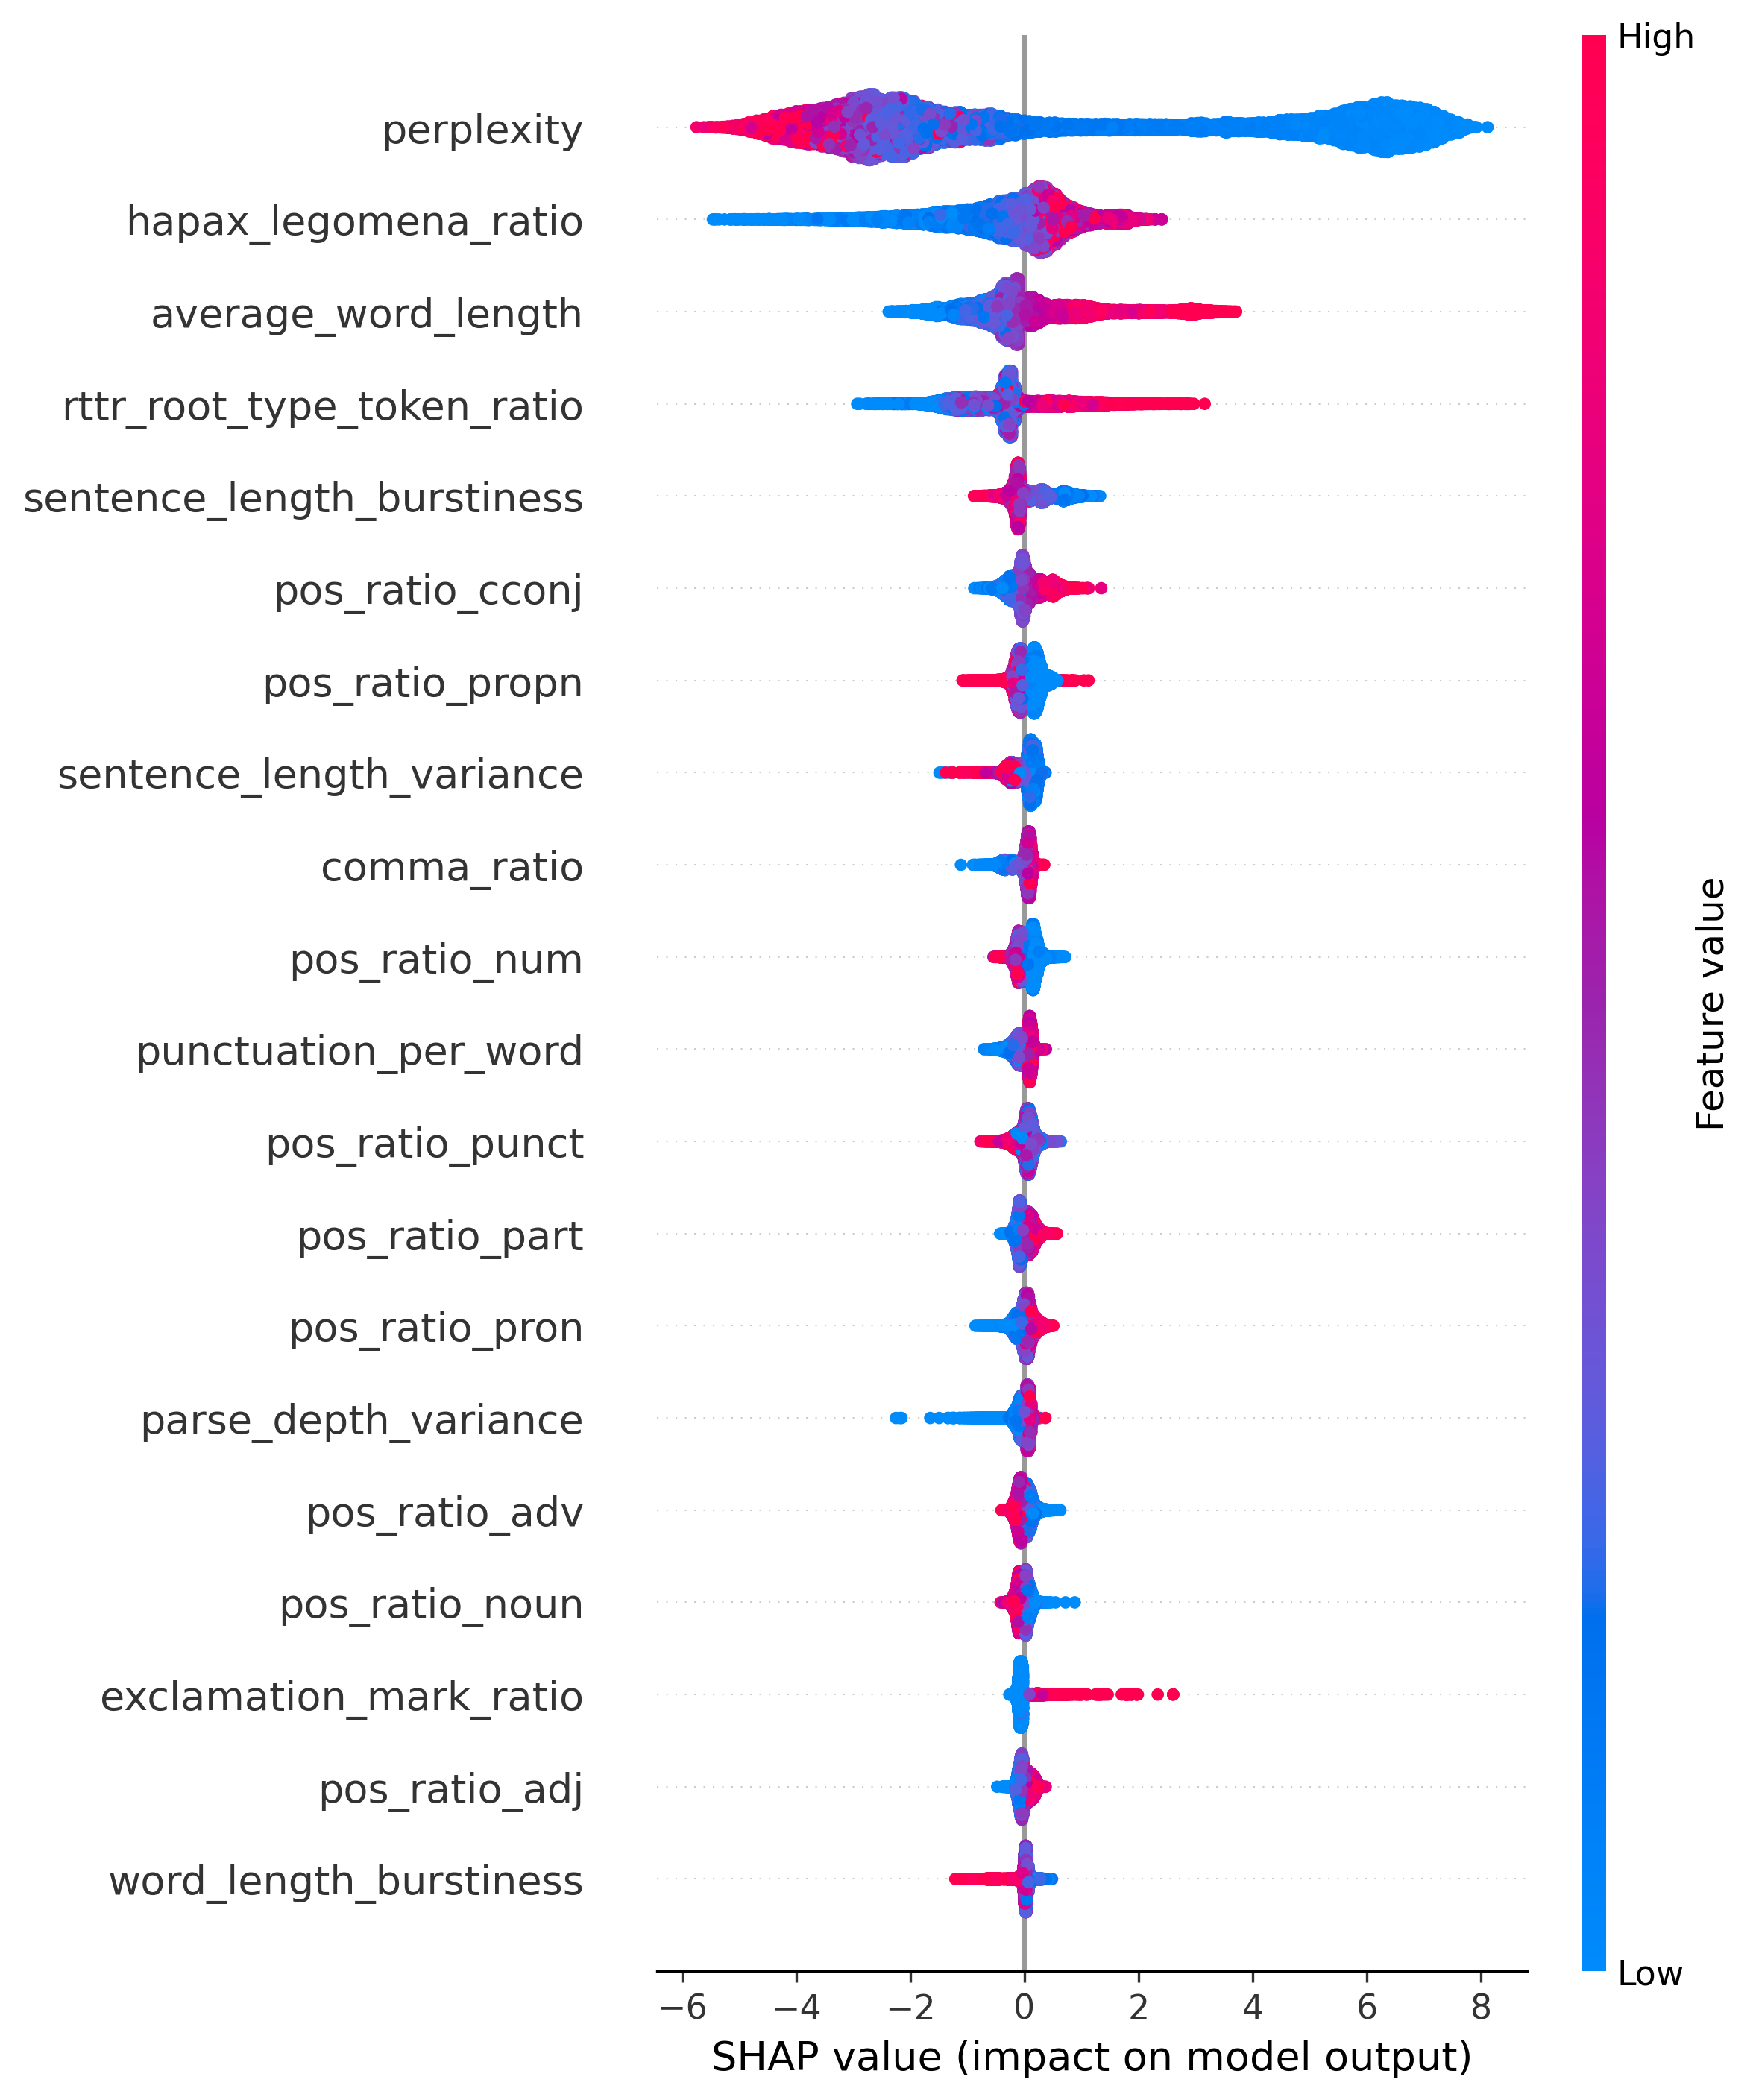
\includegraphics[width=\columnwidth]{../plots/shap_plot.png}
\caption{SHAP summary plot for XGBoost classifier. Positive values indicate AI-generated}
\label{fig:shap-summary}
\end{figure}

\subsection{Ensemble Classifier}
\label{sec:ensemble-classifier}

Table \ref{tab:within-dataset-ensemble} presents the within-dataset performance of all classifiers in the ensemble-based detector on the held-out test set (22,570 samples). XGBoost achieved the highest individual performance (97.62\% accuracy, 0.997 AUROC), followed by DeBERTa (94.24\% accuracy, 0.988 AUROC) and BERT (91.33\% accuracy, 0.972 AUROC). The voting ensemble achieved 95.58\% accuracy, demonstrating robust aggregation across diverse classifiers, while the stacking ensemble matched XGBoost's performance (97.62\% accuracy).

\begin{table}[t]
\centering
\footnotesize
\begin{tabular}{@{}lccc@{}}
\toprule
\textbf{Classifier} & \textbf{Accuracy} & \textbf{Macro F1} & \textbf{AUROC} \\
\midrule
Random Classifier & 0.501 & 0.501 & 0.500 \\
\midrule
Naive Bayes & 0.860 & 0.860 & 0.925 \\
BERT & 0.913 & 0.913 & 0.972 \\
DeBERTa & 0.942 & 0.942 & 0.988 \\
XGBoost & \textbf{0.976} & \textbf{0.976} & \textbf{0.997} \\
\midrule
Voting Ensemble & 0.956 & 0.956 & N/A \\
Stacking Ensemble & \textbf{0.976} & \textbf{0.976} & N/A \\
\bottomrule
\end{tabular}
\caption{Within-dataset performance of ensemble component models. Best values in bold.}
\label{tab:within-dataset-ensemble}
\end{table}

The near-perfect AUROC values (0.972-0.997) indicate excellent classification performance on the within-dataset test set, with XGBoost and DeBERTa demonstrating superior discrimination capability compared to baseline methods (see Appendix \ref{sec:auroc-curves} for detailed AUROC curves).

\subsection{Cross-Dataset Evaluation}
As described in Section \ref{sec:evaluation}, we performed leave-one-dataset-out cross-validation, training on three datasets and testing on the held-out one (10,000 test samples per dataset). These results highlight a reversal in model rankings under distribution shifts. Table \ref{tab:cross-dataset-results} compares within-dataset and cross-dataset performance, revealing significant changes in relative performance across models.

\begin{table}[t]
\centering
\footnotesize
\resizebox{\columnwidth}{!}{%
\begin{tabular}{@{}lcccc@{}}
\toprule
\textbf{Model} & \textbf{Within} & \textbf{Cross} & \textbf{Change} & \textbf{Variance} \\
               & \textbf{Acc (\%)} & \textbf{Acc (\%)} & \textbf{(\%)} & \\
\midrule
XGBoost & 97.62 & 82.76 & -14.86 & ±1.83 \\
DeBERTa & 94.24 & 96.57 & +2.33 & ±0.18 \\
BERT & 91.33 & 89.26 & -2.07 & ±2.52 \\
Naive Bayes & 86.00 & 80.95 & -5.05 & ±2.14 \\
Voting Ensemble & 95.58 & 88.89 & -6.69 & ±1.49 \\
Stacking Ensemble & 97.62 & 84.43 & -13.19 & ±0.16 \\
\bottomrule
\end{tabular}
}
\caption{Within-dataset vs. cross-dataset performance comparison.}
\label{tab:cross-dataset-results}
\end{table}

Table \ref{tab:ensemble-component-results} provides detailed cross-dataset performance metrics for all classifiers. The transformer-based DeBERTa classifier achieved the highest performance (96.57\% accuracy, 0.994 AUROC), demonstrating superior generalization across domains. Among the feature-based approaches, XGBoost showed significant overfitting with 82.76\% accuracy compared to its within-dataset performance of 97.62\% (Table \ref{tab:within-dataset-ensemble}), while the voting ensemble provided robust performance (88.89\% accuracy).

\begin{table}[t]
\centering
\footnotesize
\begin{tabular}{@{}lccc@{}}
\toprule
\textbf{Classifier} & \textbf{Accuracy} & \textbf{Macro F1} & \textbf{AUROC} \\
\midrule
Random Classifier & 0.494 & 0.494 & 0.500 \\
\midrule
Naive Bayes & 0.809 & 0.775 & 0.941 \\
BERT & 0.893 & 0.884 & 0.959 \\
DeBERTa & \textbf{0.966} & \textbf{0.964} & \textbf{0.994} \\
XGBoost & 0.828 & 0.814 & 0.860 \\
Voting Ensemble & 0.889 & 0.877 & N/A \\
Stacking Ensemble & 0.844 & 0.830 & N/A \\
\bottomrule
\end{tabular}
\caption{Cross-dataset performance comparison of ensemble component models. Best values in bold.}
\label{tab:ensemble-component-results}
\end{table}

AUROC curves on held-out datasets (Appendix \ref{sec:auroc-curves}) confirm DeBERTa's superior discrimination (AUC 0.9948 and 0.9923) and XGBoost's limitations (AUC 0.7967 and 0.9224) when generalizing to unseen data.

The ensemble methods demonstrated robust performance across multiple evaluation metrics, with the voting ensemble achieving 88.89\% accuracy (±1.49\% variance) and providing consistent improvements in terms of stability and generalization across domains. Comparing to within-dataset results (Table \ref{tab:within-dataset-ensemble}), the voting ensemble maintained performance (+0.19\% change), while the stacking ensemble declined (-4.27\% change), suggesting that simple aggregation methods generalize better than complex meta-learning approaches.

Having examined both feature-based and ensemble performance, we now discuss the key findings and their implications for AI text detection.

\section{Discussion and Conclusion}
\label{sec:discussion-conclusion}
% Concisely assess your project, addressing errors and their potential causes. Discuss method limitations, dataset issues, and consider alternative approaches. Briefly explore ethical implications and societal impact of deploying your NLP solutions, suggesting ways to address ethical concerns. Summarise your conclusions.

\subsection{Feature Importance Findings}
\label{sec:feature-importance-discussion}
The consistency of perplexity as the top-ranked feature across all three models (importance scores: 0.334-0.430) indicates that perplexity captures fundamental differences in text generation patterns. As expected, the direction of this relationship is that a higher perplexity score is indicative of human-written text, i.e. that AI text is more predictable to the Pythia 1.4B model, likely because there are similarities in the training data of different LLMs.

Lexical features are also consistently among the top discriminators across all models. AI-generated text is characterized by longer words and greater vocabulary diversity. This shows that modern LLMs employ a more varied vocabulary than human writers, possibly reflecting their large and diverse training corpora, where the average human vocabulary reaches natural limits and domain constraints.

Apart from perplexity, the models show differences in the feature importance rankings. Logistic Regression and Random Forest emphasize syntactic complexity features (parse depth variance, sentence structure), while XGBoost relies on simpler POS-based features. However, cross-dataset evaluation (Table \ref{tab:cross-dataset-results}) reveals that XGBoost's high within-dataset performance (97.62\% accuracy) stems from overfitting to dataset-specific artifacts, dropping to 82.76\% on unseen data (as visualized in Figures \ref{fig:sunilthite-auroc} and \ref{fig:daigt-auroc}, where its curve shows poorer separation with AUROC 0.7967--0.9224).
This suggests that while linguistic features like perplexity remain discriminative, feature-based approaches may learn domain-specific patterns rather than general AI characteristics, limiting their real-world utility.

\subsection{Ensemble-Based Detector vs. Individual Classifiers}
\label{sec:ensemble-based-detector-discussion}
Cross-dataset evaluation (Table \ref{tab:cross-dataset-results}) reveals a fundamental tradeoff: XGBoost excels within-dataset (97.62\%) but overfits severely (-14.86 points to 82.76\% cross-dataset), while DeBERTa generalizes better (94.24\% to 96.57\%), learning robust linguistic patterns rather than dataset artifacts (Figures \ref{fig:sunilthite-auroc} and \ref{fig:daigt-auroc}). Voting ensembles provide middle-ground robustness (88.89\%) with low variance (±1.49\%), while stacking offers no benefit (84.43\%), validating simple aggregation for RQ2. Feature-based methods capture dataset-specific patterns; transformers capture generalizable characteristics.

\subsection{Method Limitations}
\label{sec:method-limitations}
Our datasets include only pure human-written or AI-generated samples, lacking mixed or adversarially modified text. Robustness to evasion techniques requires further evaluation before deployment. Additionally, datasets lack non-English text and text from latest LLMs (GPT-5, Claude Sonnet 4.5, Gemini 2.5 Pro), representing primarily academic essays and Q\&A from pre-2024 models (GPT-3.5, GPT-4). Performance may degrade on contemporary text distributions (social media, code) and newer model generations, necessitating continuous retraining.

The perplexity feature uses a single model (Pythia 1.4B trained on the Pile), limiting generalizability to LLMs with different training distributions. Within-dataset evaluation overestimated XGBoost's effectiveness; cross-dataset testing proved essential for realistic assessment.

\textbf{Computational Considerations:} While transformers require more resources than feature-based approaches, XGBoost's computational advantage is limited by perplexity calculation requiring GPU-accelerated Pythia 1.4B inference. This accuracy-efficiency tradeoff matters for resource-constrained deployments.

\subsection{Ethical and Societal Considerations}
\label{sec:ethical-considerations}
This project develops an AI detection tool, which can be used to detect AI-generated text in a range of domains such as academia, journalism or creative writing. Our intention is that knowledge about whether a text is AI-generated or not can be used in a "positive" way for society in general. In the mentioned domains, this could be help prevent fraud in academic settings, or help journalists flag sources that may be AI-generated and require further investigation. Our tool explicitly tackles the problem of adversarial attacks against AI-detection tools by using an ensemble of classifiers where one will have to fool multiple models to successfully fool the tool. However, it is important to reflect upon how such a tool can be used to improve and create adversarial attacks/tools, both against this specific tool, but also against AI-detectors in general, by training an adversarial model by using this tool in a detector-evasion setup.

Another ethical consideration is that this tool does not have zero false positive or false negative rates. Incorrect classification of human-written text can have serious consequences for the individual, such as a student being accused of cheating, possibly leading to failing a course or even being expelled from a university. Incorrect classification of AI-generated text on the other hand can lead to spread of misinformation such as "fake" news or made up scientific findings with a "stamp" of authenticity. To minimize these potential harms, a tool such as this should be deployed with transparent confidence scores and clear disclaimers and explanations about its limitations. 

\subsection{Conclusion}
\label{sec:conclusion}
Perplexity and lexical features (average word length, hapax legomena ratio) are most discriminative for AI-text detection (RQ1), but transformers like DeBERTa (96.57\% cross-dataset) generalize far better than feature-based XGBoost (82.76\%), which overfits to dataset artifacts. Voting ensembles enhance robustness (88.89\%) compared to individual classifiers (RQ2), though stacking offers no benefit. Cross-dataset evaluation proved essential—within-dataset metrics alone (XGBoost: 97.62\%) misleadingly suggest reliability where severe overfitting exists.

For practical deployment, prioritize DeBERTa for cross-domain robustness; use XGBoost only when training and deployment distributions match. Cross-dataset validation is critical before deployment. Given ethical risks (false positives in academic settings, adversarial misuse), deploy with transparent confidence scores and human oversight. Future work should investigate adversarial robustness, domain adaptation, and why transformers generalize better than feature-based methods.

\balance

\bibliographystyle{acl_natbib}
\bibliography{references}


\appendix
\section*{Appendix}

\section{Dataset Details}
\label{sec:dataset-details}

\subsection{Dataset Class Distributions}
Table \ref{tab:dataset-class-distribution} shows the original class distributions across the four datasets used in this study, before balancing.

\begin{table}[H]
\centering
\footnotesize
\begin{tabular}{lrcc}
\toprule
\textbf{Dataset} & \textbf{Samples} & \textbf{Human (\%)} & \textbf{AI (\%)} \\
\midrule
HC3 & 85K & 68.5 & 31.5 \\
sunilthite & 29K & 60.1 & 39.9 \\
DAIGT V2 & 45K & 61.0 & 39.0 \\
AH\&AITD & 12K & 50.0 & 50.0 \\
\bottomrule
\end{tabular}
\caption{Dataset size and class distributions before balancing}
\label{tab:dataset-class-distribution}
\end{table}

\subsection{Combined Dataset Composition}
Table \ref{tab:combined-dataset} shows the final composition of the combined balanced dataset used for training and evaluation.

\begin{table}[H]
\centering
\footnotesize
\begin{tabular}{lrr}
\toprule
\textbf{Dataset} & \textbf{Samples} & \textbf{Proportion (\%)} \\
\midrule
HC3 & 43,000 & 38.1 \\
DAIGT V2 & 34,994 & 31.0 \\
sunilthite & 23,274 & 20.6 \\
AH\&AITD & 11,580 & 10.3 \\
\midrule
\textbf{Total} & \textbf{112,848} & \textbf{100.0} \\
\bottomrule
\end{tabular}
\caption{Combined dataset composition after balancing}
\label{tab:combined-dataset}
\end{table}

\section{AUROC Curves}
\label{sec:auroc-curves}

\subsection{Within-Dataset AUROC Curves}
Figure \ref{fig:within-dataset-roc} shows the AUROC curves for all classifiers on the within-dataset test set (22,570 samples). The curves illustrate the superior discrimination capability of XGBoost (AUC 0.997) and DeBERTa (AUC 0.988) compared to baseline methods. The near-perfect AUROC values indicate excellent classification performance when models are tested on data from the same distribution as training.

\begin{figure*}[t]
\centering
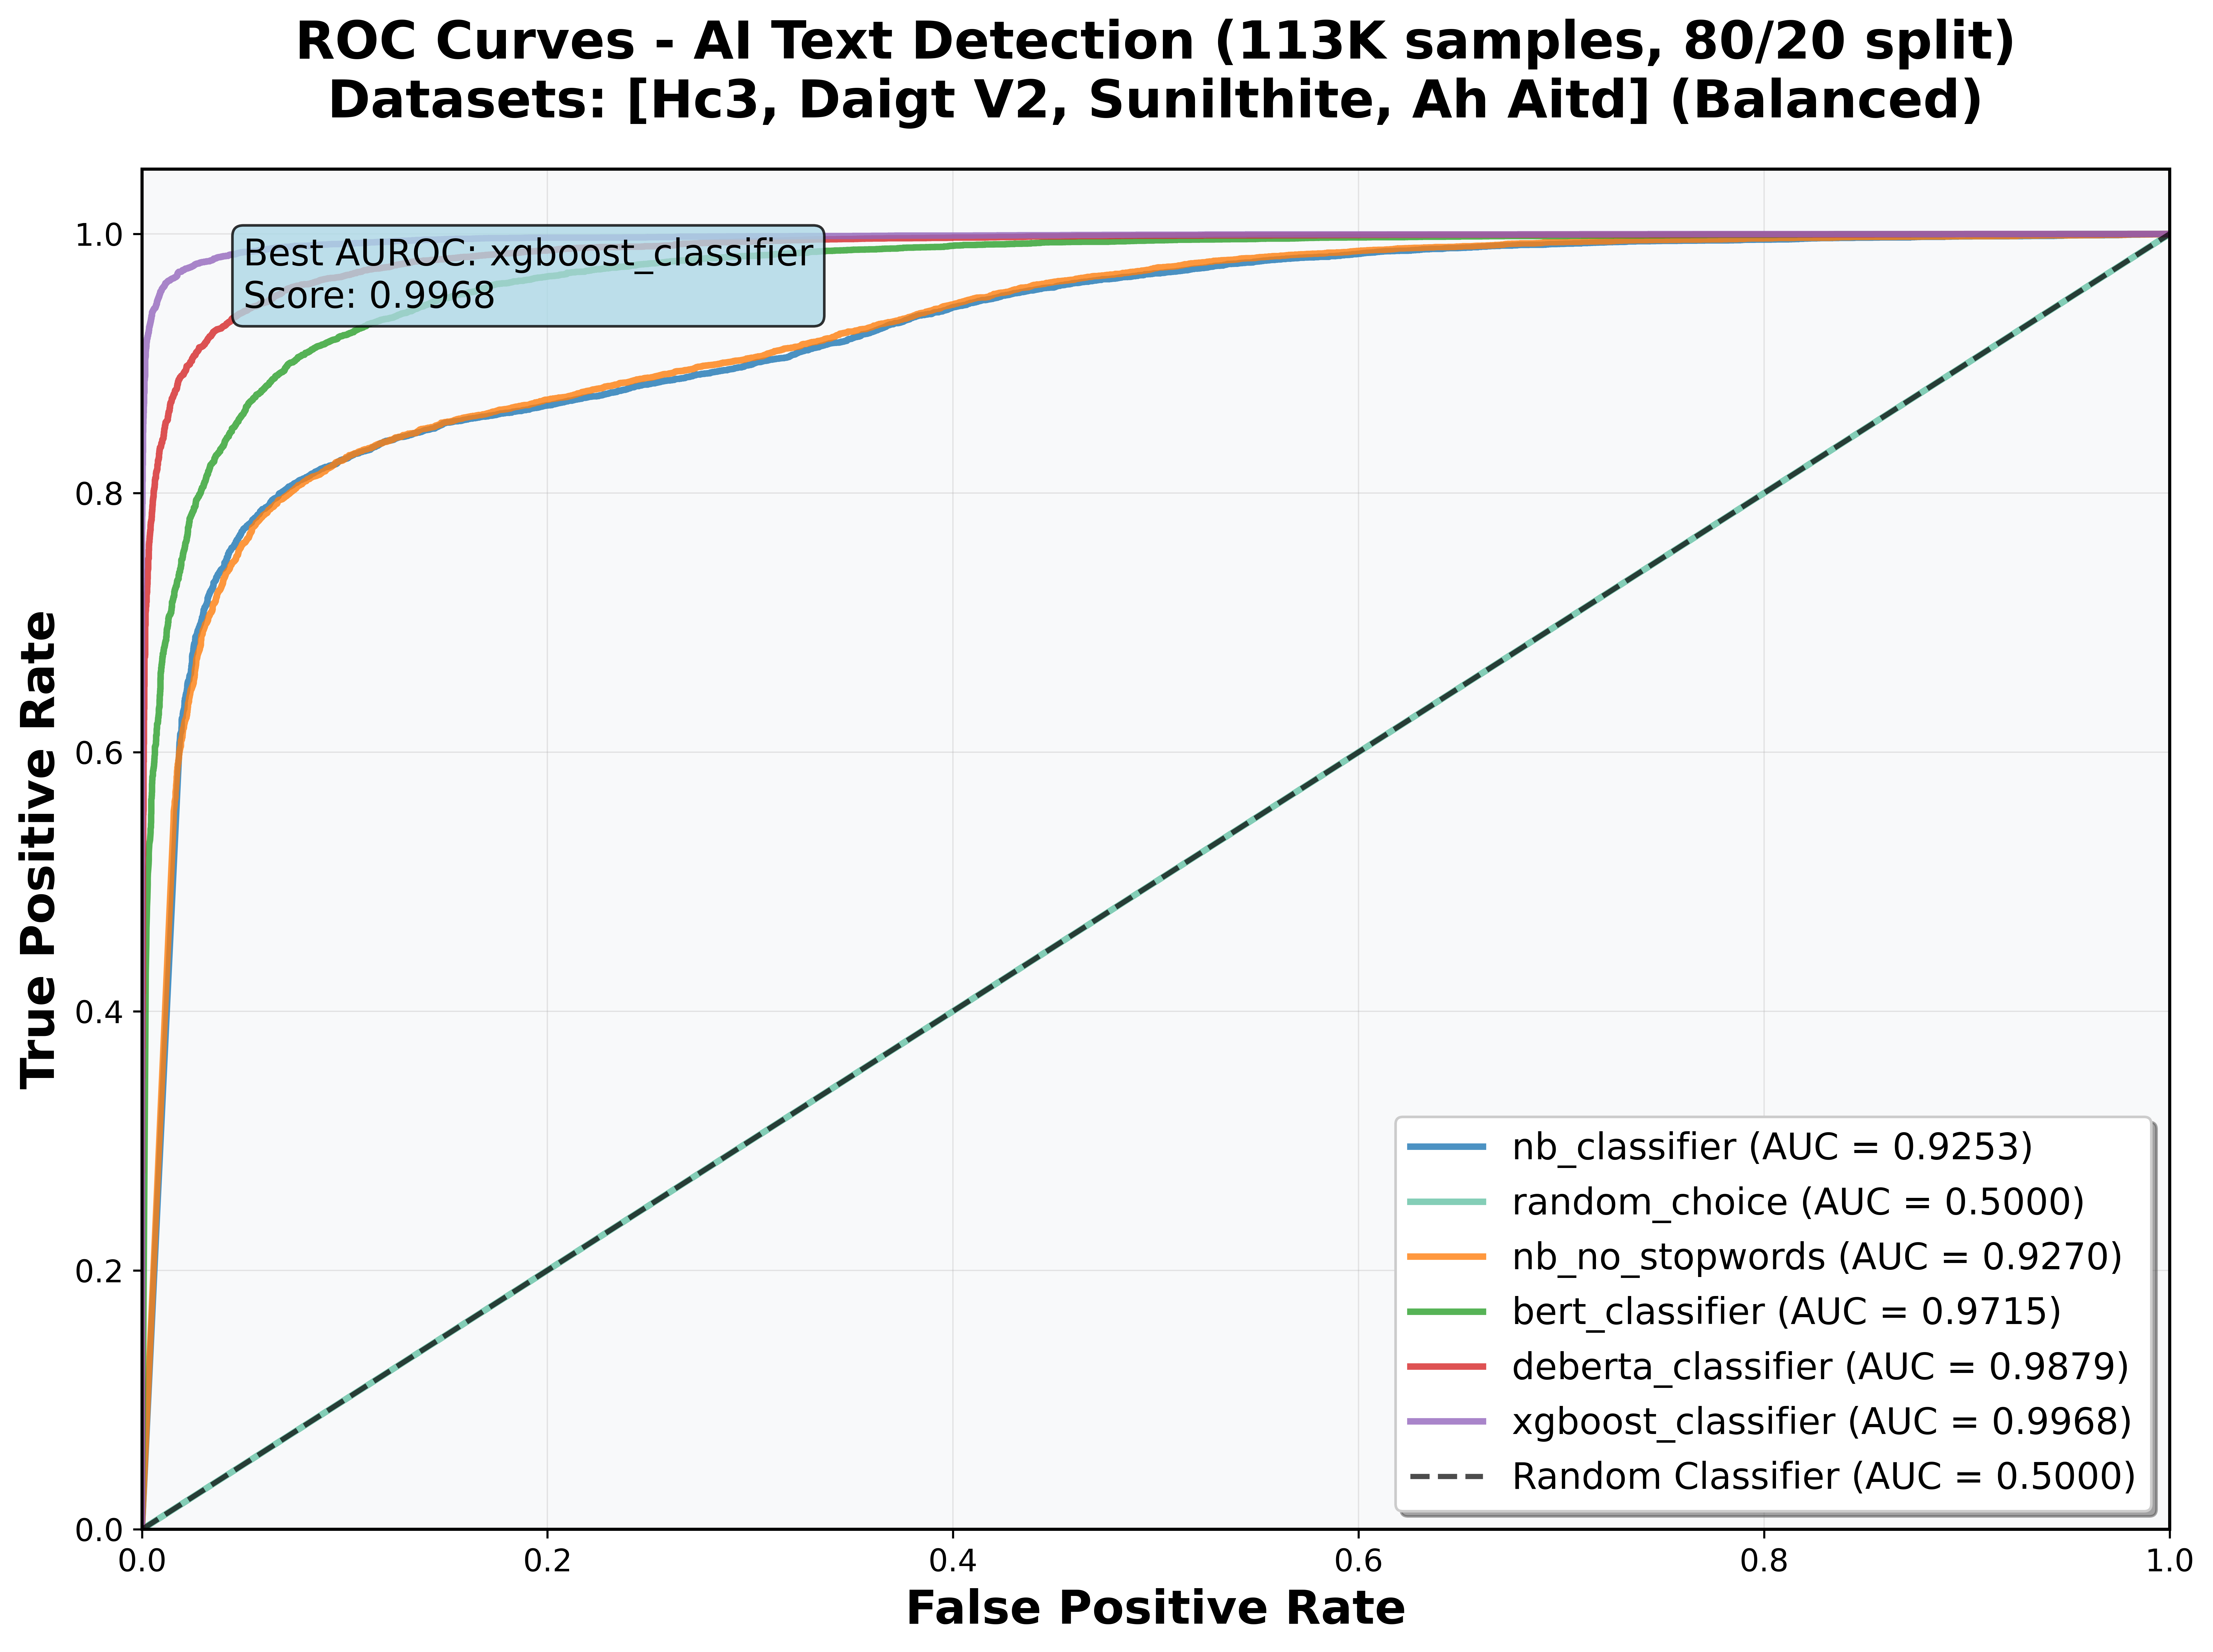
\includegraphics[width=0.6\textwidth]{20-10-poster-results/roc_curves_20251020_185318.png}
\caption{AUROC curves for all classifiers on within-dataset test set.}
\label{fig:within-dataset-roc}
\end{figure*}

\subsection{Cross-Dataset AUROC Curves}
Figures \ref{fig:sunilthite-auroc} and \ref{fig:daigt-auroc} show AUROC curves on held-out datasets from leave-one-dataset-out cross-validation. These curves reveal significant performance differences when models face distribution shifts: DeBERTa maintains superior discrimination (AUC 0.9948 and 0.9923), while XGBoost shows substantial degradation (AUC 0.7967 and 0.9224), confirming its overfitting to training dataset characteristics.

\begin{figure*}[t]
\centering
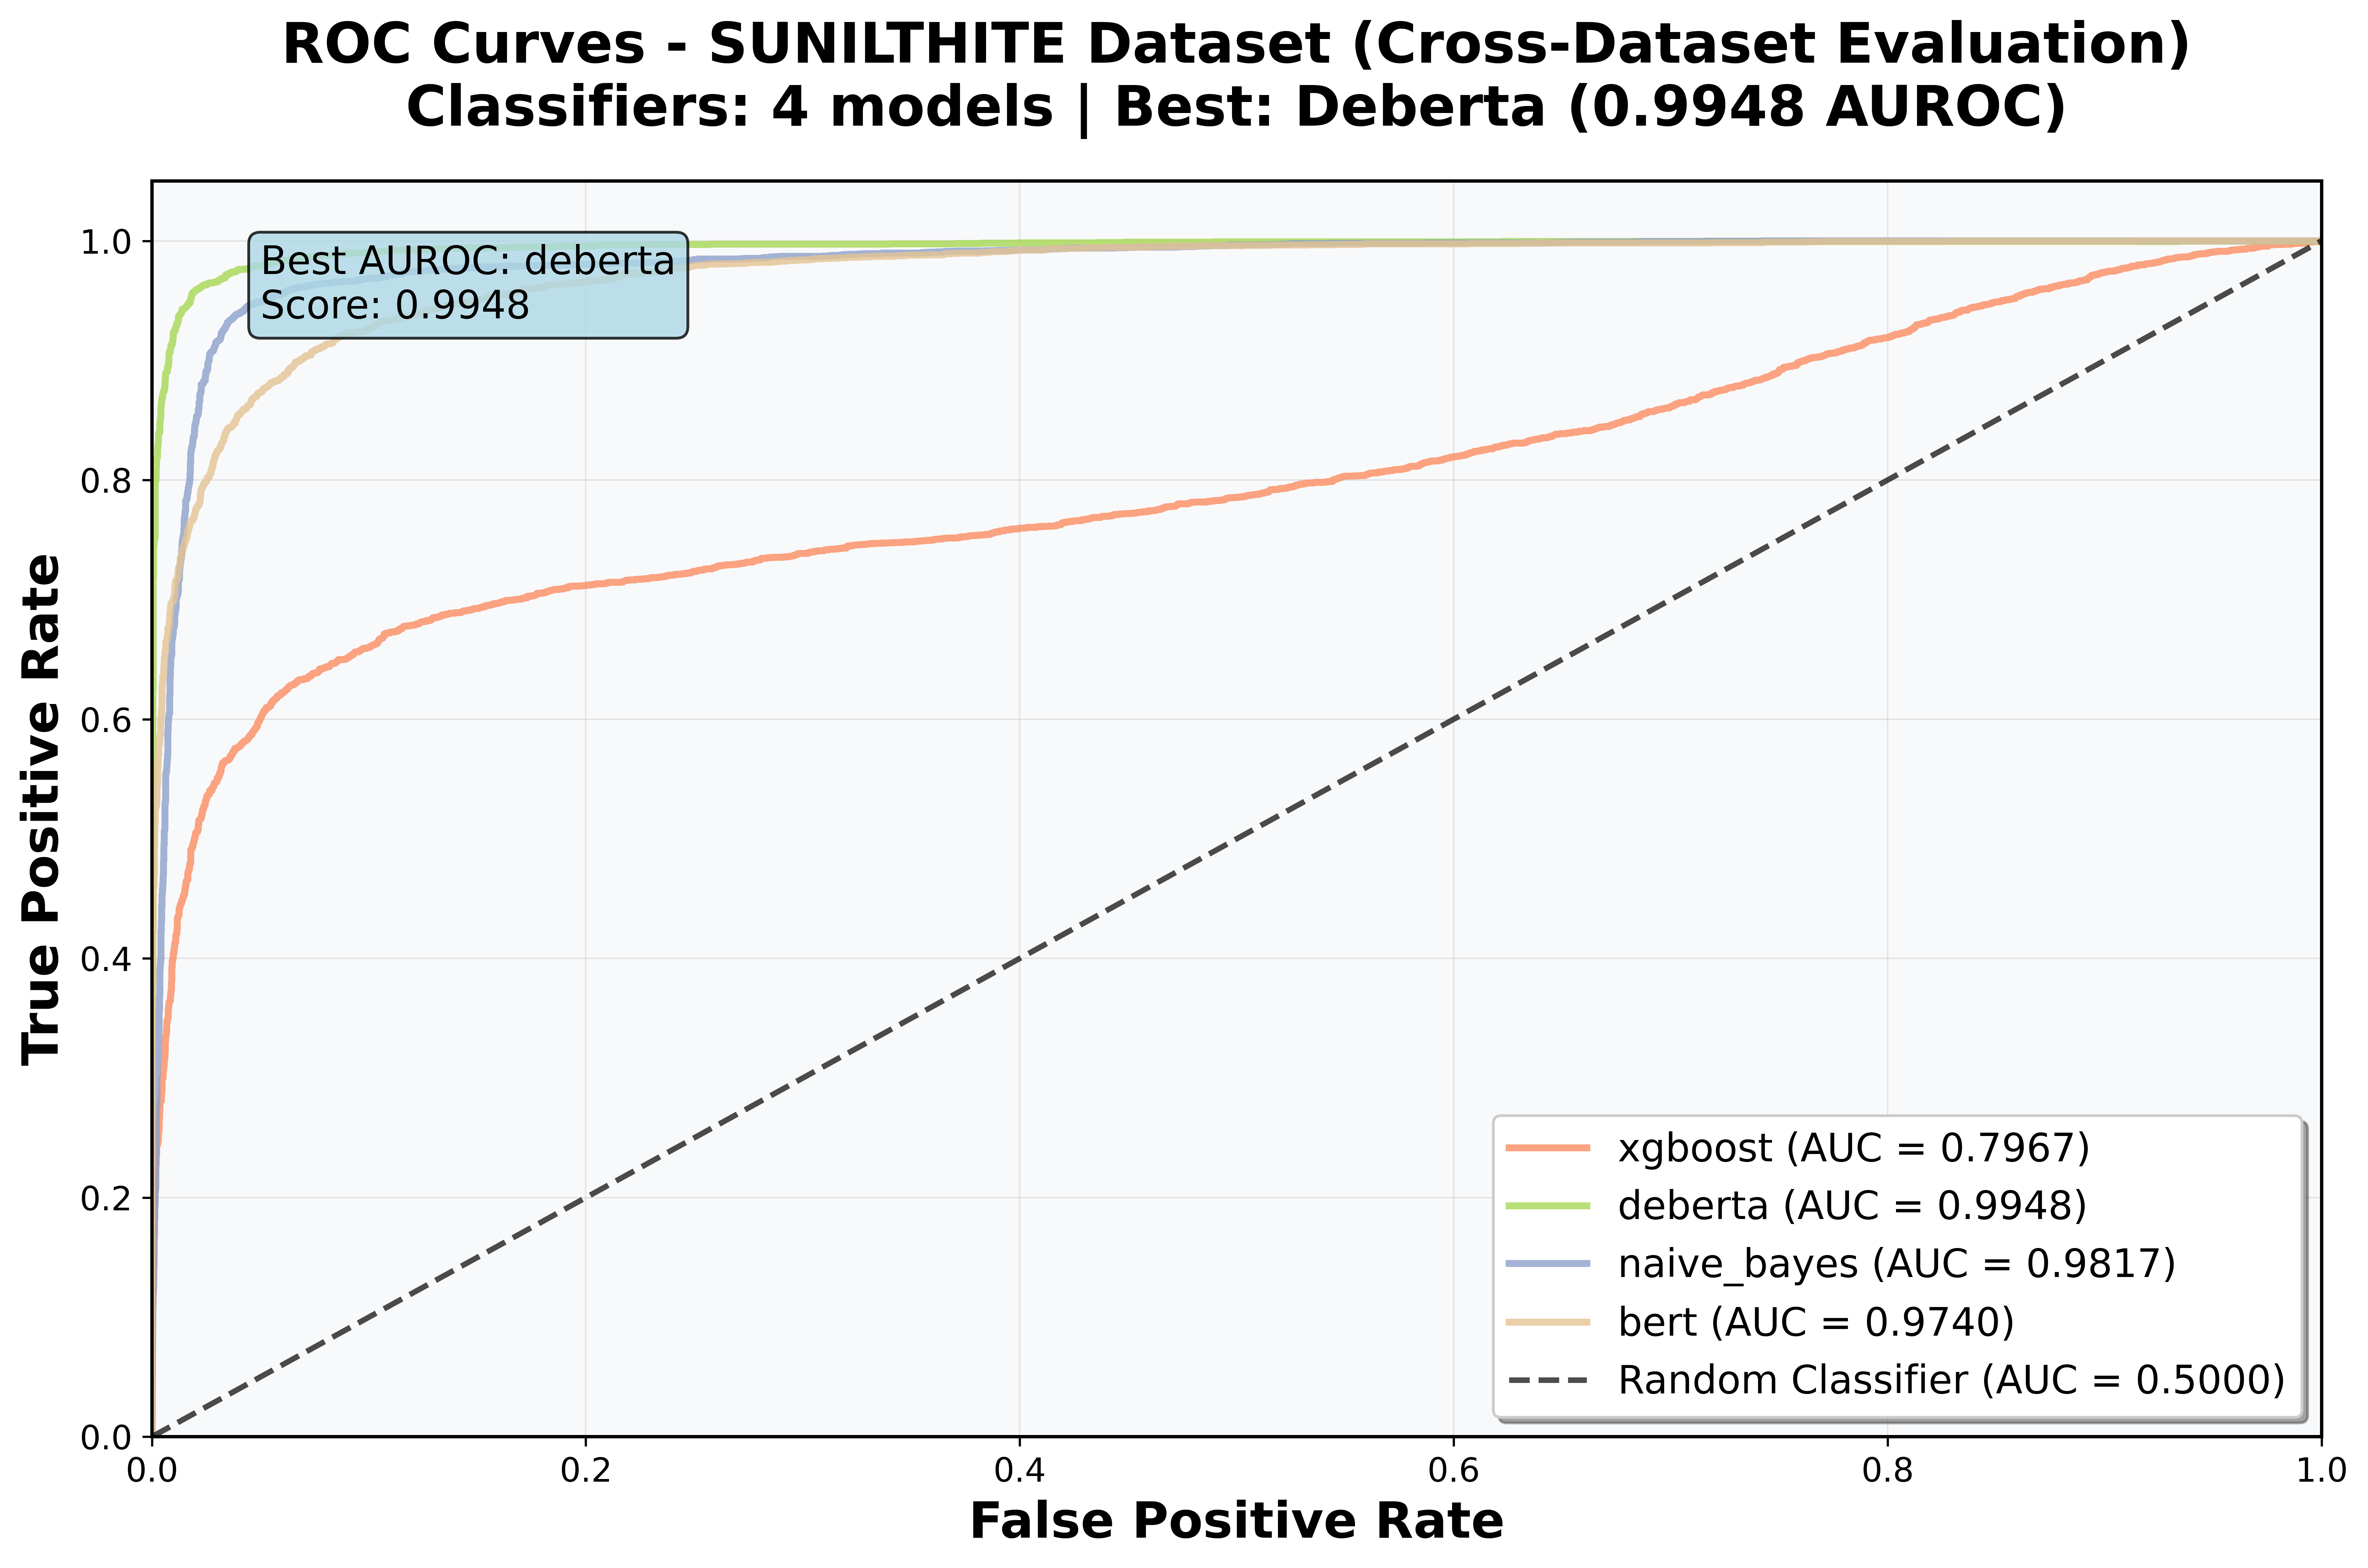
\includegraphics[width=0.5\textwidth]{7-11-crossdataset-results/roc_curves_sunilthite_20251107_211231.png}
\caption{AUROC curves for models on the SUNILTHITE held-out dataset.}
\label{fig:sunilthite-auroc}
\end{figure*}

\begin{figure*}[t]
\centering
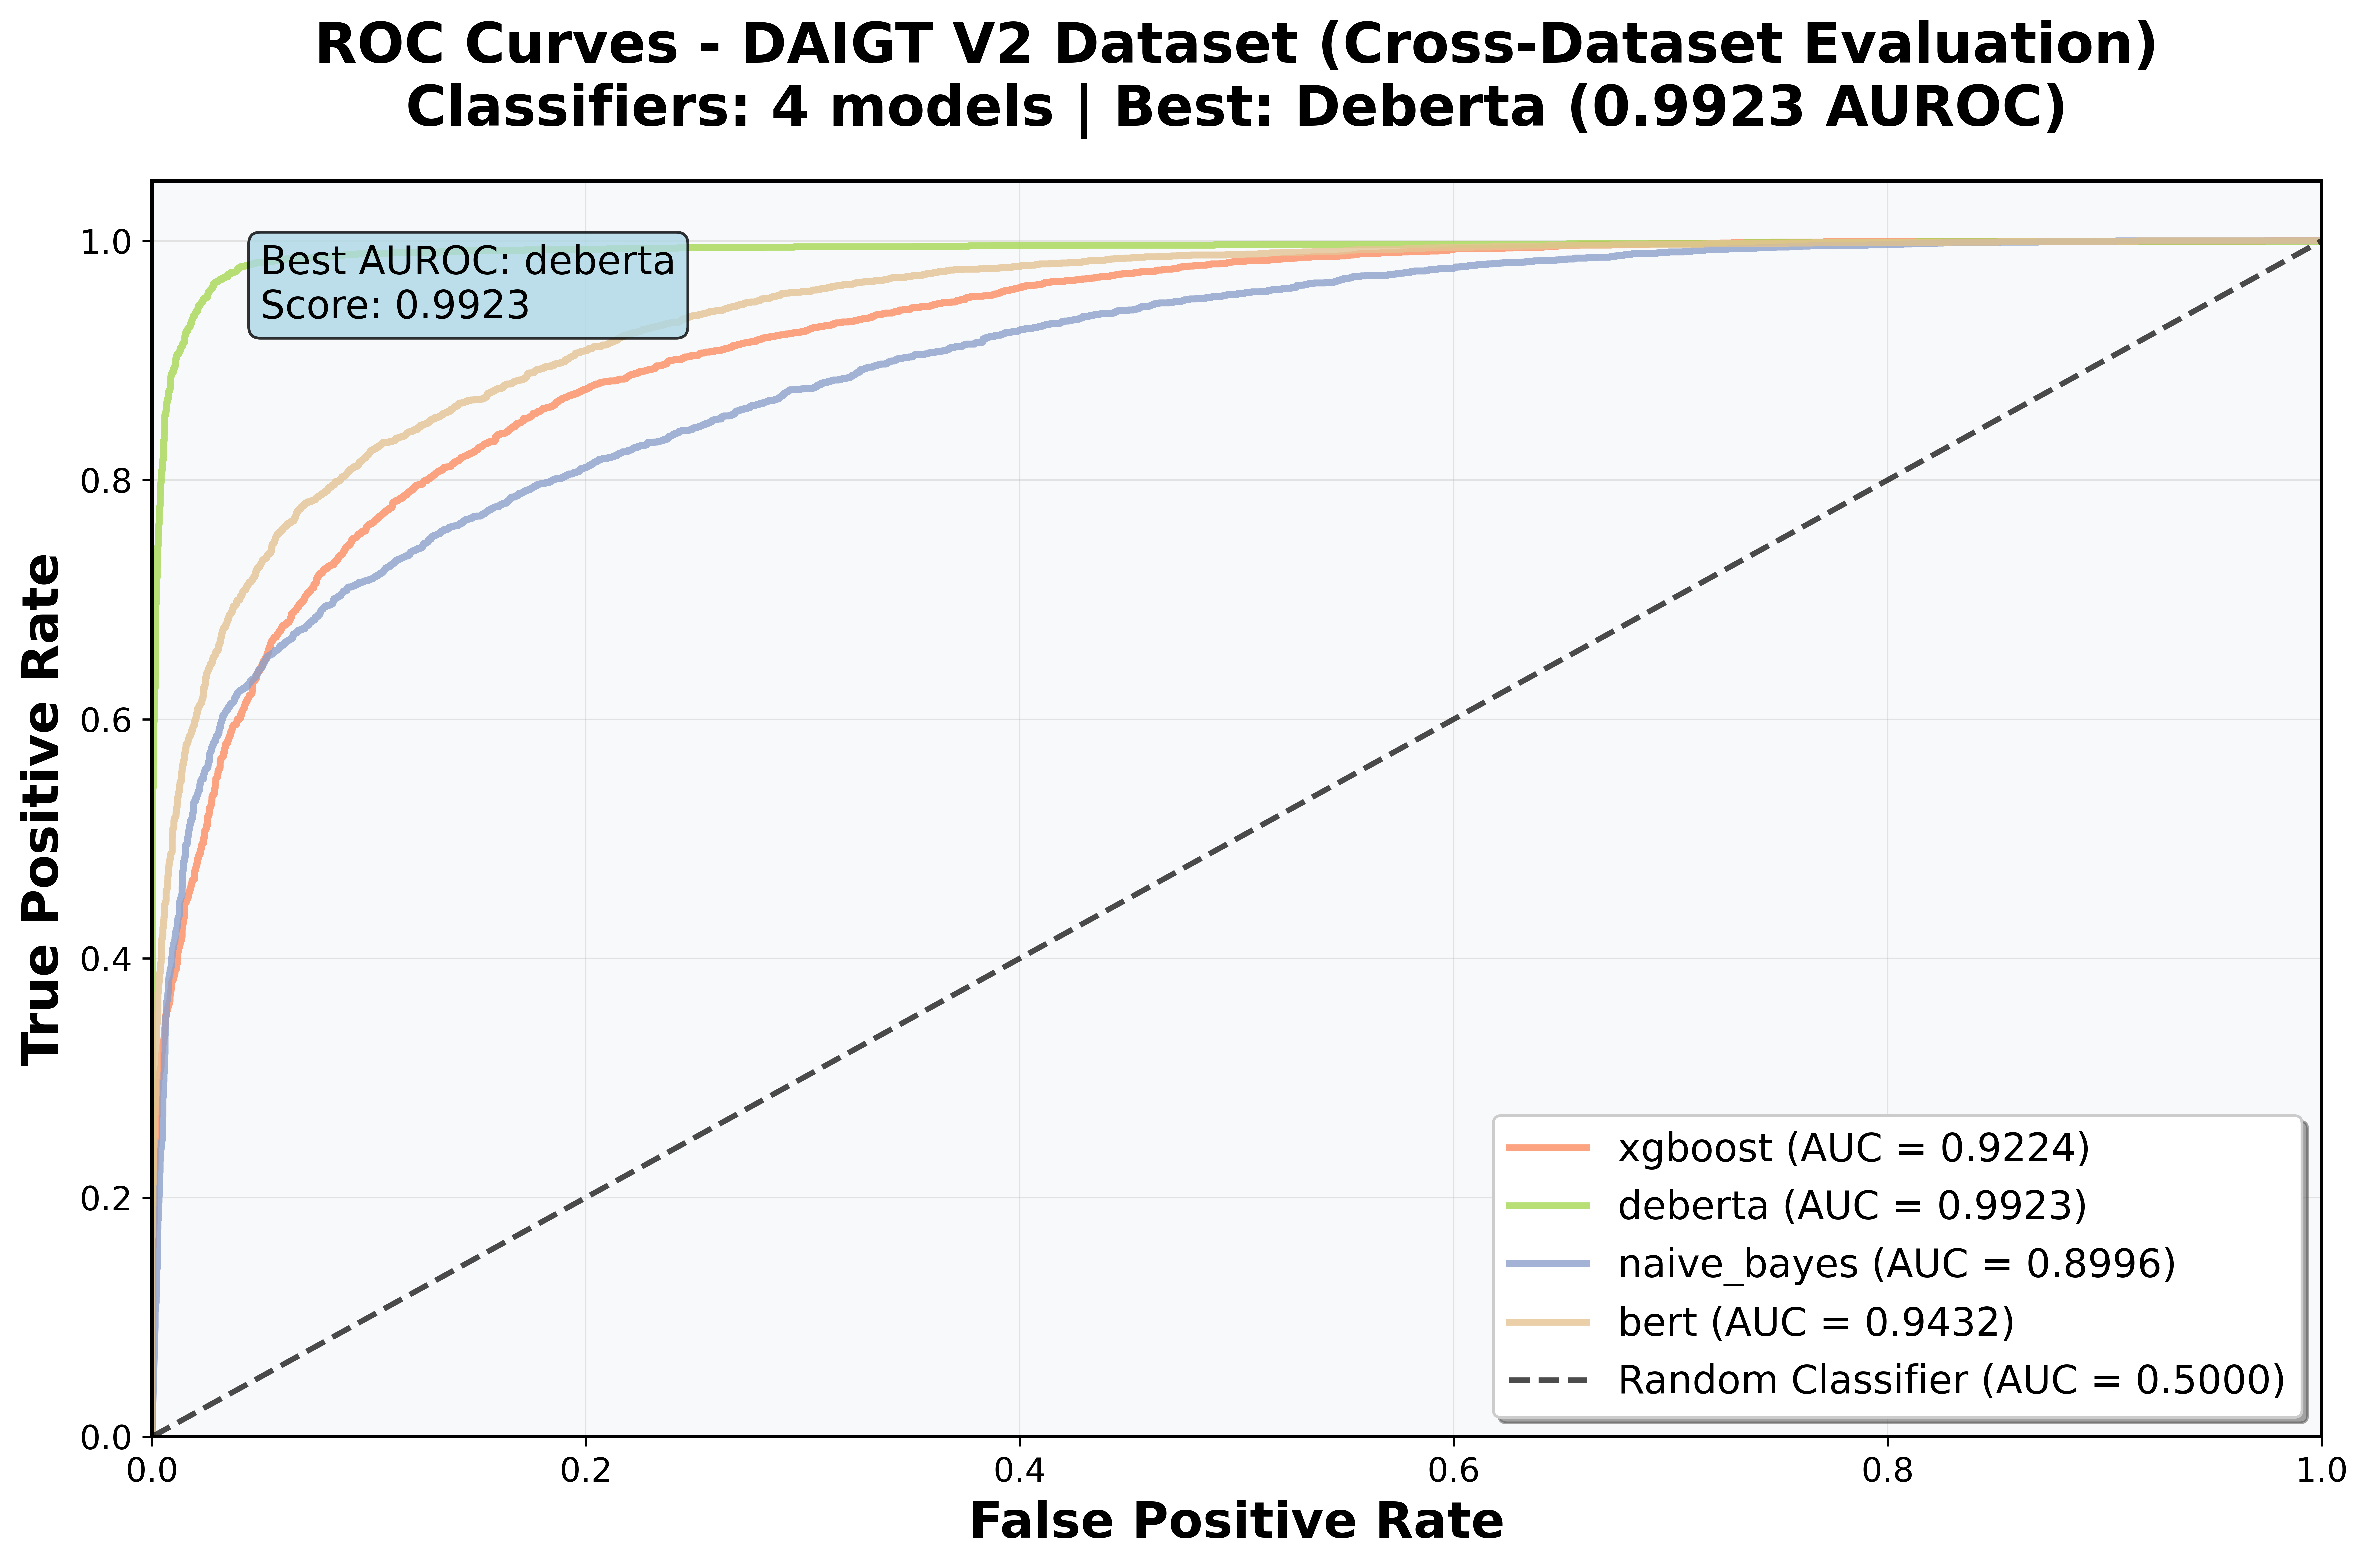
\includegraphics[width=0.6\textwidth]{7-11-crossdataset-results/roc_curves_daigt_v2_20251107_211231.png}
\caption{AUROC curves for models on the DAIGT V2 held-out dataset.}
\label{fig:daigt-auroc}
\end{figure*}

\section{Full List of Extracted Features}
\label{sec:full-list-of-features}

{\footnotesize\ttfamily
average\_word\_length, word\_length\_variance, rttr\_root\_type\_token\_ratio, hapax\_legomena\_ratio, average\_sentence\_length, sentence\_length\_variance, average\_parse\_depth, maximum\_parse\_depth, parse\_depth\_variance, comma\_ratio, period\_ratio, exclamation\_mark\_ratio, question\_mark\_ratio, punctuation\_per\_word, pos\_ratio\_adj, pos\_ratio\_adp, pos\_ratio\_adv, pos\_ratio\_aux, pos\_ratio\_conj, pos\_ratio\_cconj, pos\_ratio\_det, pos\_ratio\_intj, pos\_ratio\_noun, pos\_ratio\_num, pos\_ratio\_part, pos\_ratio\_pron, pos\_ratio\_propn, pos\_ratio\_punct, pos\_ratio\_sconj, pos\_ratio\_sym, pos\_ratio\_verb, pos\_ratio\_x, noun\_to\_verb\_ratio, sentence\_length\_burstiness, sentence\_length\_iqr, position\_burstiness\_diff, long\_sentence\_ratio, word\_length\_burstiness, clause\_length\_burstiness, perplexity
}

\end{document}
